\subsection{CANONICAL BILINEAR FORM}

We have seen (no. 1, Prop. 3) that the symmetric bilinear form

\[
(x, y) \mapsto \mathrm{B} _ {\mathrm{R}} (x, y) = \sum_ {\alpha \in \mathbb {R}} \langle \alpha^ {\prime}, x \rangle \langle \alpha^ {\prime}, y \rangle
\]

on V is non-degenerate and invariant under A(R). Interchanging the roles of R and \(R^{\prime}\), it follows that the symmetric bilinear form \((x^{*}, y^{*}) \mapsto \mathrm{B}_{\mathbb{R}^{\prime}}(x^{*}, y^{*}) = \sum_{\alpha \in \mathbb{R}^{\prime}} \langle \alpha, x^{*} \rangle \langle \alpha, y^{*} \rangle\) on \(V^{*}\) is non-degenerate and invariant under A(R).

The inverse form of \(B_{R^{\prime}}\) (resp. \(B_{R}\) ) on V (resp. \(V^{*}\) ) will be called the canonical bilinear form on V (resp. \(V^{*}\) ) and denoted by \(\Phi_{R}\) (resp. \(\Phi_{R^{\prime}}\) ). It is non-degenerate and invariant under A(R). Let \(\sigma\) be the isomorphism from V to \(V^{*}\) defined by \(B_{R^{\prime}}\) . Then, for \(x \in V\) and \(y \in V\) :

\[
\Phi_ {R} (x, y) = B _ {R ^ {\prime}} (\sigma (x), \sigma (y)) = \sum_ {\alpha \in R} \langle \alpha , \sigma (x) \rangle \langle \alpha , \sigma (y) \rangle .
\]

But \(\langle \alpha, \sigma(x) \rangle = B_{R^{\prime}}(\sigma(\alpha), \sigma(x)) = \Phi_R(\alpha, x)\) . Hence,

\[
\Phi_ {\mathsf {R}} (x, y) = \sum_ {\alpha \in \mathsf {R}} \Phi_ {\mathsf {R}} (\alpha , x) \Phi (\alpha , y).\tag{16}
\]

In view of Prop. 7 of no. 2, \(\Phi_{R}\) is the only non-zero symmetric bilinear form invariant under W(R) which satisfies the identity (16).

For \(\beta \in \mathbb{R}\) , (16) gives

\[
\varPhi_ {\mathrm{R}} (\beta , \beta) = \sum_ {\alpha \in \mathrm{R}} \varPhi_ {\mathrm{R}} (\alpha , \beta) ^ {2} = \frac {1}{4} \varPhi_ {\mathrm{R}} (\beta , \beta) ^ {2} \sum_ {\alpha \in \mathrm{R}} n (\alpha , \beta) ^ {2},
\]

hence

\[
4 \Phi_ {R} (\beta , \beta) ^ {- 1} = \sum_ {\alpha \in R} n (\alpha , \beta) ^ {2}.\tag{17}
\]

Moreover, by Lemma 2 of no. 1, we have, for \(x, y \in V\) :

\[
\begin{array}{r l} & {\mathrm{B} _ {\mathrm{R}} (x, y) = \sum_ {\alpha \in \mathrm{R}} \varPhi_ {\mathrm{R}} \left(\frac {2 \alpha}{\varPhi_ {\mathrm{R}} (\alpha , \alpha)}, x\right) \left(\frac {2 \alpha}{\varPhi_ {\mathrm{R}} (\alpha , \alpha)}, y\right)} \\ & {\qquad = 4 \sum_ {\alpha \in \mathrm{R}} \varPhi_ {\mathrm{R}} (\alpha , x) \varPhi_ {\mathrm{R}} (\alpha , y) \varPhi_ {\mathrm{R}} (\alpha , \alpha) ^ {- 2}.} \end{array}
\]

It follows that, if \(R\) is irreducible, there exists a constant \(\gamma(R) > 0\) such that

\[
\sum_ {\alpha \in R} \Phi_ {R} (\alpha , x) \Phi_ {R} (\alpha , y) \Phi_ {R} (\alpha , \alpha) ^ {- 2} = \gamma (R) \Phi_ {R} (x, y).\tag{18}
\]

By the definition of \(\gamma (\mathbb{R})\) , we have \(B_{\mathbb{R}}(x,y) = 4\gamma (\mathbb{R})\Phi_{\mathbb{R}}(x,y)\) , so

\[
\Phi_ {\mathrm{R} ^ {\prime}} \left(x ^ {*}, y ^ {*}\right) = (4 \gamma (\mathrm{R})) ^ {- 1} \mathrm{B} _ {\mathrm{R} ^ {\prime}} \left(x ^ {*}, y ^ {*}\right)
\]

for \(x^{*},y^{*}\in V^{*}\) . This proves that \(\gamma (\mathsf{R}) = \gamma (\mathsf{R}^{\prime})\) . On the other hand, for \(\beta \in \mathbb{R}\) ,

\[
\begin{array}{c} \Phi_ {\mathrm{R} ^ {\prime}} (\beta^ {\prime}, \beta^ {\prime}) = (4 \gamma (\mathrm{R})) ^ {- 1} \sum_ {\alpha \in \mathfrak {R}} \langle \beta^ {\prime}, \alpha \rangle^ {2} \\ = \gamma (\mathrm{R}) ^ {- 1} \sum_ {\alpha \in \mathbb {R}} \frac {\Phi_ {\mathrm{R}} (\alpha , \beta) ^ {2}}{\Phi_ {\mathrm{R}} (\beta , \beta) ^ {2}} \end{array}
\]

so, by (16),

\[
\Phi_ {\mathrm{R} ^ {\prime}} (\beta^ {\prime}, \beta^ {\prime}) = \gamma (\mathrm{R}) ^ {- 1} \Phi_ {\mathrm{R}} (\beta , \beta) ^ {- 2} \Phi_ {\mathrm{R}} (\beta , \beta)
\]

or finally

\[
\Phi_ {R} (\beta , \beta) \Phi_ {R ^ {\prime}} (\beta^ {\prime}, \beta^ {\prime}) = \gamma (R) ^ {- 1}.\tag{19}
\]

Further, if all the roots of \(\mathbb{R}\) have the same length \(\lambda\) for \(\varPhi_{\mathbb{R}}\) , (16) and (18) show that

\[
\gamma (R) = \lambda^ {- 4}.\tag{20}
\]

Moreover, if \(h\) is the Coxeter number of \(W\) , the Cor. of Th. 1 of Chap. V, § 6, no. 2 shows that:

\[
h \Phi_ {R} (x, x) = \sum_ {\alpha \in R} \left(x, \frac {\alpha}{\lambda}\right) ^ {2} \text {   for   all   } x \in V.
\]

Comparing with (16), we deduce that

\[
\lambda = h ^ {- 1 / 2} \text { or } \gamma (\mathrm{R}) = h ^ {2}.\tag{21}
\]

Finally, formula (19) shows that the roots of \(R^{\prime}\) have length \(\lambda\) for \(\Phi_{R^{\prime}}\) .

\section{AFFINE WEYL GROUP}

In this paragraph (except in no. 5), we denote by R a reduced root system in a real vector space V. We denote by W the Weyl group of R; we identify it with a group of automorphisms of the dual \(V^{*}\) of V ( \(\S\) 1, no. 1), and we provide \(V^{*}\) with a scalar product invariant under W. Let E be the affine space underlying \(V^{*}\) ; for \(v \in V^{*}\) , we denote by \(t(v)\) the translation of E by the vector v. Finally, we denote by P (resp. Q) the group of translations \(t(v)\) whose vector v belongs to the group of weights \(\mathrm{P}(\mathrm{R}^{\prime})\) (resp. to the group of radical weights \(\mathrm{Q}(\mathrm{R}^{\prime})\) ) of the inverse root system \(R^{\prime}\) of R.

\subsection{AFFINE WEYL GROUP}

For \(\alpha \in \mathbb{R}\) and \(k\in \mathbf{Z}\) , let \(\mathrm{L}_{\alpha ,k}\) be the hyperplane of E defined by:

\[
\mathrm{L} _ {\alpha , k} = \{x \in \mathrm{E} | \langle \alpha , x \rangle = k \}
\]

and let \(s_{\alpha, k}\) be the orthogonal reflection with respect to \(L_{\alpha, k}\) . Then

\[
s _ {\alpha , k} (x) = x - (\langle \alpha , x \rangle - k) \alpha^ {\prime} = s _ {\alpha , 0} (x) + k \alpha^ {\prime}
\]

for all \(x \in E\) . In other words,

\[
s _ {\alpha , k} = t (k \alpha^ {\prime}) \circ s _ {\alpha}\tag{1}
\]

where \(s_{\alpha}\) is the orthogonal reflection with respect to the hyperplane \(L_{\alpha} = L_{\alpha,0}\) , i.e.~the reflection associated to the root \(\alpha\) .

Formula (1) shows that \(s_{\alpha, k}\) does not depend on the choice of scalar product.

DEFINITION 1. The group of affine transformations of E generated by the reflections \(s_{\alpha,k}\) for \(\alpha \in R\) and \(k \in Z\) is called the affine Weyl group of the root system R and denoted by \(\mathrm{W}_{a}(\mathrm{R})\) (or simply by \(W_{a}\) ).

PROPOSITION 1. The group \(\mathrm{W}_a\) is the semi-direct product of \(\mathrm{W}\) by \(\mathrm{Q}\) .

Since W is generated by the reflections \(s_{\alpha}\) , it is contained in \(W_{a}\) . On the other hand, \(t(\alpha^{\prime}) = s_{\alpha,1} \circ s_{\alpha}\) if \(\alpha \in R\) , which shows that \(Q \subseteq W_{a}\) .

Since W leaves \(Q(R^{\prime})\) stable ( \(\S\) 1, no. 9), the group G of affine transformations generated by W and Q is the semi-direct product of W by Q. Now \(G \subseteq W_{a}\) from above and \(s_{\alpha,k} \in G\) for all \(\alpha \in R\) and \(k \in Z\) by (1). It follows that \(W_{a} = G\) .

PROPOSITION 2. The group \(W_{a}\) , with the discrete topology, acts properly on E and permutes the hyperplanes \(L_{\alpha,k}\) (for \(\alpha \in R\) and \(k \in Z\) ).

Since \(Q(R^{\prime})\) is a discrete subgroup of \(V^{*}\) , the group Q acts properly on E. Hence, so does \(W_{a} = W.Q\) , since W is finite. Moreover, for \(\alpha, \beta \in R\) and \(k \in Z\) :

\[
s _ {\beta} (\mathrm{L} _ {\alpha , k}) = \mathrm{L} _ {\gamma , k} \text {with} \gamma = s _ {\beta} (\alpha) \in \mathrm{R},
\]

\[
t (\beta^ {\prime}) \left(\mathrm{L} _ {\alpha , k}\right) = \mathrm{L} _ {\alpha , k + n (\alpha , \beta)},
\]

where \(n(\alpha, \beta) = \langle \beta^{\prime}, \alpha \rangle\) is an integer, hence the second assertion.

We can thus apply the results of Chapter V, § 3 to \(W_{a}\) acting on E. To avoid any confusion with the chambers of the Weyl group W in \(V^{*}\) , we shall call the chambers determined by the system of hyperplanes \(L_{\alpha,k}\) (for \(\alpha \in R\) and \(k \in Z\) ) in E alcoves. The group \(W_{a}\) thus acts simply transitively on the set of alcoves and the closure of an alcove is a fundamental domain for \(W_{a}\) acting on E (Chap. V, § 3, no. 2, Th. 1 and no. 3, Th. 2). It is clear that the Weyl group W is identified with the canonical image \(U(W_{a})\) of \(W_{a}\) in the orthogonal group of \(V^{*}\) (cf.~Chap. V, § 3, no. 6). It follows that \(W_{a}\) is essential (Chap. V, § 3, no. 7) and that \(W_{a}\) is irreducible if and only if the root system R is (§ 1, no. 2, Cor. of Prop. 5). If R is irreducible, every alcove is an open simplex (Chap. V, § 3, no. 9, Prop. 8). In the general case, the canonical product decomposition of the affine space E (Chap. V, § 3, no. 8) corresponds to the decomposition of R into irreducible components. In particular, the alcoves are products of open simplexes.

Note also that the Cor. of Th. 1 of Chap. V, § 3, no. 2 shows that the \(s_{\alpha,k}\) are the only reflections in \(\mathbf{W}_a\) .

\subsection{WEIGHTS AND SPECIAL WEIGHTS}

PROPOSITION 3. The special points (Chap. V, § 3, no. 10, Def. 1) of \(W_{a}\) are the weights of \(R^{\prime}\) .

Let \(x_0 \in E\) and let \(\alpha \in R\) . The hyperplane L parallel to Ker \(\alpha\) and passing through \(x_0\) has equation \(\langle \alpha, x \rangle = \langle \alpha, x_0 \rangle\) . To be equal to some \(L_{\beta,k}\) , it is necessary on the one hand that \(\alpha\) and \(\beta\) are proportional, and so, since R is reduced, that \(\beta = \pm \alpha\) , and on the other hand that \(\langle \alpha, x_0 \rangle\) is an integer. It follows immediately that \(x_0\) is a special point of \(W_a\) if and only if \(\langle \alpha, x_0 \rangle \in Z\) for all \(\alpha \in R\) , in other words, if and only if \(x_0 \in P(R^{\prime})\) (§ 1, no. 9).

COROLLARY. (i) If \(\overline{\omega} \in \mathrm{P}(\mathbb{R}^{\prime})\) , there exists an alcove C such that \(\overline{\omega}\) is an extremal point of \(\overline{\mathbb{C}}\) .

\begin{enumerate}
\def\labelenumi{(\roman{enumi})}
\setcounter{enumi}{1}
\tightlist
\item
  If \(\mathbf{C}\) is an alcove, \(\overline{\mathbf{C}} \cap \mathbf{Q}(\mathbb{R}^{\prime})\) reduces to a single point and this is an extremal point of \(\overline{\mathbf{C}}\) .
\end{enumerate}

This follows from Prop. 3, in view of the Cor. of Prop. 11 of Chap. V, § 3, no. 10 and Prop. 12 of Chap. V, § 3, no. 10.

PROPOSITION 4. Let \(C'\) be a chamber of \(R'\) .

\begin{enumerate}
\def\labelenumi{(\roman{enumi})}
\item
  There exists a unique alcove C contained in \(\mathbf{C}'\) such that \(0\in \overline{\mathbf{C}}\)
\item
  The union of the \(w(\overline{\mathbf{C}})\) for \(w\in \mathrm{W}\) is a neighbourhood of 0 in E.
\item
  Every wall of \(\mathbf{C}'\) is a wall of \(\mathbf{C}\) .
\end{enumerate}

This follows from Prop. 11 of Chap. V, § 3, no. 10.

Assume now that \(R\) is irreducible. Let \((\alpha_i)_{i\in I}\) be a basis of \(R\) (§1, no. 5, Def. 2), and let \((\overline{\omega}_i)_{i\in I}\) be the dual basis. The \(\overline{\omega}_i\) are the fundamental weights of \(R^{\prime}\) for the chamber \(D'\) of \(R^{\prime}\) corresponding to the basis \((\alpha_i)\) . Let

\[
\tilde {\alpha} = \sum_ {i \in \mathrm{I}} n _ {i} \alpha_ {i}
\]

be the highest root of \(\mathbf{R}\) (§ 1, no. 8), and let \(\mathbf{J}\) be the set of \(i \in \mathbf{I}\) such that \(n_i = 1\) .

PROPOSITION 5. Let \(\mathbf{C}\) be the alcove contained in \(\mathbf{C}'\) and containing 0 in its closure (Prop. 4).

\begin{enumerate}
\def\labelenumi{(\roman{enumi})}
\tightlist
\item
  C is the set of \(x \in E\) such that \(\langle\alpha_{i}, x\rangle > 0\) for all \(i \in I\) and \(\langle\tilde{\alpha}, x\rangle < 1\) .
\item
  The set \(\overline{C} \cap P(R^{\prime})\) consists of 0 and the \(\overline{\omega}_{i}\) for \(i \in J\) .
\end{enumerate}

Let D be the set of \(x \in E\) such that \(\langle\tilde{\alpha}, x\rangle < 1\) and set \(C_{1} = C' \cap D\) . Since \(0 \in \overline{C}\) , we have \(C \subseteq D\) and hence \(C \subseteq C_{1}\) . We are going to show that, for all \(\alpha \in R\) and all \(k \in Z\) , the sets C and \(C_{1}\) are on the same side of the hyperplane \(L_{\alpha,k}\) . This will prove that \(C_{1} \subseteq C\) and so will establish assertion (i). If k = 0, the whole of the chamber \(C'\) is on one side of \(L_{\alpha,0}\) , which establishes our assertion in this case. If \(k \neq 0\) , we may, by replacing \(\alpha\) by \(-\alpha\) , assume that k \textgreater{} 0. Then \(\langle\alpha, x\rangle < k\) on C, since \(0 \in \overline{C}\) . On the other hand, \(\tilde{\alpha} - \alpha\) is positive on \(C'\) (§ 1, no. 8, Prop. 25). Thus, for \(y \in C_{1}\) , we have \(\langle\alpha, y\rangle \leqslant \langle\tilde{\alpha}, y\rangle < 1 \leqslant k\) . Consequently, C and \(C_{1}\) are on the same side of \(L_{\alpha,k}\) .

Now let \(\overline{\omega} \in P(R^{\prime})\) . Then \(\overline{\omega} = \sum_{i} p_i \overline{\omega}_i\) , with \(p_i \in \mathbf{Z}\) (§ 1, no. 10), and \(\overline{\omega} \in \overline{C'}\) if and only if the integers \(p_i\) are positive. If \(\overline{\omega} \in \overline{C'}\) , then \(\overline{\omega} \in \overline{C}\) if and only if \(\langle \tilde{\alpha}, \overline{\omega} \rangle = \sum_{i} n_i p_i\) is \(\leqslant 1\) , hence (ii).

COROLLARY. The alcove C is an open simplex with vertices 0 and the \(\overline{\omega}_i / n_i\) , \(i \in I\) .

This follows from (i).

\subsection{\texorpdfstring{NORMALISER OF \(W_{a}\)}{NORMALISER OF W\_a}}

In this no., we assume that the chosen scalar product on V is invariant not only under W but under the whole of the group A(R). We identify A(R) and A(R \(^{\prime}\) ).

Let G be the normaliser of \(W_{a}\) in the group of displacements of the affine euclidean space E. If g is a displacement of E, and s is the orthogonal reflection with respect to a hyperplane L, the displacement \(gsg^{-1}\) is the orthogonal reflection with respect to the hyperplane \(g(L)\) . It follows that G is the set of displacements of E that permute the hyperplanes \(L_{\alpha,k}\) (for \(\alpha \in R\) and \(k \in Z\) ).

Now, the group of automorphisms of E is the semi-direct product of the orthogonal group U of \(V^{*}\) and the group T of translations. If \(u \in U\) and \(v \in V^{*}\) , the hyperplane \(L_{\alpha,k}\) is transformed by \(g = u \circ t(v)\) into the hyperplane with equation

\[
\langle^ {t} u ^ {- 1} (\alpha), x \rangle = k + \langle \alpha , v \rangle .
\]

Consequently, \(g \in \mathbf{G}\) if and only if, on the one hand \({}^t u\) permutes the roots, in other words belongs to \(\mathrm{A(R)}\) , and on the other hand \(\langle \alpha, v \rangle \in \mathbf{Z}\) for all \(\alpha \in \mathbb{R}\) , that is \(v \in \mathrm{P(R^{\prime})}\) . In other words, the group \(G\) is the semi-direct product of \(A(R)\) by \(P\) . Since \(Q \subseteq P\) and \(W \subseteq A(R)\) , the quotient group \(G / W_a\) is the semi-direct product of \(A(R)/W\) by \(P(R^{\prime})/Q(R^{\prime})\) ; it is immediately checked that the corresponding action of \(A(R)/W\) on \(P(R^{\prime})/Q(R^{\prime})\) is the canonical action (§1, no. 9).

We denote by \(W_{a}^{\prime}\) the subgroup of G formed by the semi-direct product of W by P. This is a normal subgroup of G, and \(G/W_{a}^{\prime}\) is canonically isomorphic to \(A(R)/W\) ; moreover, the canonical map from \(P(R^{\prime})\) to \(W_{a}^{\prime}/W_{a}\) gives by passing to the quotient an isomorphism from \(P(R^{\prime})/Q(R^{\prime})\) to \(W_{a}^{\prime}/W_{a}\) .

Now let C be an alcove of E, and let \(G_{C}\) be the subgroup consisting of the elements \(g \in G\) such that \(g(\mathrm{C}) = \mathrm{C}\) . Since \(W_{a}\) is simply-transitive on the alcoves, the group G is the semi-direct product of \(G_{C}\) by \(W_{a}\) . The corresponding isomorphism from \(G/W_{a}\) to \(G_{C}\) gives rise in particular to a canonical isomorphism from \(\mathrm{P}(\mathrm{R}^{\prime})/\mathrm{Q}(\mathrm{R}^{\prime})\) to the group \(\Gamma_{C} = G_{C} \cap W_{a}^{\prime}\) .

Assume that R is irreducible, and retain the notation of Prop. 5 of no. 2. Put \(R_{0} = R\) , and let \(R_{i} (i \in I)\) be the root system generated by the \(a_{j}\) , for \(j \neq i\) . For i = 0 (resp. \(i \in I\) ), let \(w_{i}\) be the unique element of \(W(R_{i})\) (identified with a subgroup of W) which transforms the positive roots of \(R_{i}\) relative to the basis \((\alpha_{j})_{j \neq i}\) into negative roots (§ 1, no. 6, Cor. 3 of Prop. 17).

PROPOSITION 6. For all \(i \in \mathbf{J}\) , the element \(\gamma_i = t(\overline{\omega}_i)w_i w_0\) belongs to \(\Gamma_{C}\) and the map \(i \mapsto \gamma_i\) is a bijection from \(\mathbf{J}\) to \(\Gamma_{C} - \{1\}\) .

We remark first of all that the root \(w_{i}(\tilde{\alpha})\) is of the form

\[
n _ {i} \alpha_ {i} + \sum_ {j \neq i} b _ {i j} \alpha_ {j},
\]

and hence is positive.

We show that, if \(i \in \mathrm{J}\) , then \(\gamma_i \in \Gamma_{C}\) . Indeed, let \(a \in \mathrm{C}\) and \(b = \gamma_i(a)\) . For \(1 \leqslant j \leqslant l\) and \(j \neq i\) ,

\[
\begin{array}{r l} \langle b, \alpha_ {j} \rangle & = \langle \overline {{\omega}} _ {i} + w _ {i} w _ {0} (a), \alpha_ {j} \rangle \\ & = \langle w _ {0} (a), w _ {i} (\alpha_ {j}) \rangle > 0 \end{array}\tag{2}
\]

since \(w_0(a) \in -\mathbf{C}'\) and \(w_i(\alpha_j)\) is negative. On the other hand,

\[
\langle b, \alpha_ {i} \rangle = 1 + \left\langle w _ {0} (a), w _ {i} (\alpha_ {i}) \right\rangle \geqslant 1 + \left\langle w _ {0} (a), \tilde {\alpha} \right\rangle > 0\tag{3}
\]

since \(w_0(a) \in -\mathbf{C}'\) , \(\tilde{\alpha} - w_i(\alpha_i)\) takes negative values on \(-\mathbf{C}'\) , and \(\langle w_0(a), \tilde{\alpha} \rangle > -1\) . Finally,

\[
\langle b, \tilde {\alpha} \rangle = n _ {i} + \left\langle w _ {0} (a), w _ {i} (\tilde {\alpha}) \right\rangle = 1 + \left\langle w _ {0} (a), w _ {i} (\tilde {\alpha}) \right\rangle <   1\tag{4}
\]

since \(w_0(a) \in -\mathbf{C}'\) and \(w_i(\tilde{\alpha})\) is a positive root. The relations (2), (3) and (4) then imply that \(b \in \mathbf{C}\) , and hence that \(\gamma_i \in \Gamma_{C}\) . It is clear that the map \(i \mapsto \gamma_i\) is injective, since \(\gamma_i(0) = \overline{\omega}_i\) . Finally, let \(\gamma \in \Gamma_{C}\) with \(\gamma \neq 1\) , and put \(\gamma = tw\) with \(t \in \mathbf{P}\) and \(w \in W\) . Then \(t \neq 1\) since \(\Gamma_{C} \cap W = \{1\}\) . On the other hand, \(t(0) = \gamma(0) \in \overline{\mathbf{C}} \cap P(\mathbf{R}^{\prime})\) and Prop. 5 implies that there exists \(i \in J\) such that \(t(0) = \overline{\omega}_i\) . Then \(\gamma_i^{-1}\gamma(0) = 0\) , hence \(\gamma = \gamma_i\) since \(\Gamma_{C} \cap W = \{1\}\) . This completes the proof.

COROLLARY. The \((\bar{\omega}_i)_{i\in J}\) form a system of representatives in \(\mathrm{P}(\mathbb{R}^{\prime})\) of the non-zero elements of \(\mathrm{P}(\mathbb{R}^{\prime}) / \mathrm{Q}(\mathbb{R}^{\prime})\) .

Indeed, if we identify \(\Gamma_{C}\) with \(\mathrm{P}(\mathbb{R}^{\prime}) / \mathrm{Q}(\mathbb{R}^{\prime})\) , the element \(\gamma_{i}\) is identified with the class of \(\overline{\omega}_{i}\) mod. \(\mathrm{Q}(\mathbb{R}^{\prime})\) .

Remarks. 1) The map \(\gamma \mapsto \gamma(0)\) is a bijection from \(\Gamma_{C}\) to \(\overline{\mathrm{C}} \cap \mathrm{P}(\mathrm{R}^{\prime})\) .

\begin{enumerate}
\def\labelenumi{\arabic{enumi})}
\setcounter{enumi}{1}
\tightlist
\item
  The group G is also the normaliser of \(W_{a}\) in the group of automorphisms of E provided only with its affine structure (cf.~Exerc. 3).
\end{enumerate}

\subsection{APPLICATION: ORDER OF THE WEYL GROUP}

Lemma 1. Let X be a locally compact space countable at infinity, G a group acting continuously and properly on X, \(\mu\) a measure on X invariant under G, G' a subgroup of G, U and U' two open subsets of X with finite non-zero measure. Assume that the sU for \(s \in G\) (resp. the \(s'U'\) for \(s' \in G'\) ) are pairwise disjoint and that their union is of negligible complement. Then G' is of finite index in G and \((\mathrm{G} : \mathrm{G}') = \mu(\mathrm{U}') / \mu(\mathrm{U})\) .

Let \((s_{\lambda})_{\lambda \in \Lambda}\) be a family of representatives of the right cosets of \(G'\) in G. Let \(U_1\) be the union of the \(s_{\lambda}U\) . Then the \(s'U_1\) , for \(s' \in G'\) , are pairwise disjoint and have union \(M = \bigcup_{s \in G} sU\) . Let \(M' = \bigcup_{s' \in G'} s'U'\) . The union of \(U'\) (resp. \(U_1\) ) and a suitable subset of \(X - M'\) (resp. \(X - M\) ) is a fundamental domain, evidently \(\mu\) -measurable, for \(G'\) . By Integration, Chap. VII, § 2, no. 10, Cor. of Th. 4, \(\mu(U') = \mu(U_1)\) . This proves that \(\text{Card } \Lambda = (G : G')\) is finite, and that \(\mu(U') = (\text{Card } \Lambda)\mu(U)\) .

PROPOSITION 7. Assume that R is irreducible. Let \(B = \{\alpha_{1}, \ldots, \alpha_{l}\}\) be a basis of R, f the connection index of R (§ 1, no. 9) and \(\tilde{\alpha} = n_{1}\alpha_{1} + \cdots + n_{l}\alpha_{l}\) the highest root of R (for the order defined by B). Then the order of W is equal to

\[
(l!) n _ {1} n _ {2} \dots n _ {l} f.
\]

Let \((\overline{\omega}_{1},\ldots,\overline{\omega}_{l})\) be the basis of P(R \(^{\prime}\) ) dual to B. By the Cor. of Prop. 5, the open simplex C with vertices \(0,n_{1}^{-1}\overline{\omega}_{1},\ldots,n_{l}^{-1}\overline{\omega}_{l}\) is an alcove of E. Choose a Haar measure \(\mu\) on the additive group V*. Let A be the set of elements of V* of the form \(\xi_{1}\overline{\omega}_{1}+\cdots+\xi_{l}\overline{\omega}_{l}\) , with \(0<\xi_{i}<1\) for \(i=1,\ldots,l\) . By Cor. 2 of Prop. 15 of Integration, Chap. VII, § 1, no. 10,

\[
\mu (\mathrm{A}) / \mu (\mathrm{C}) = (l!) n _ {1} n _ {2} \dots n _ {l}.\tag{5}
\]

On the other hand, let \(A'\) be the set of elements of \(V^{*}\) of the form

\[
\xi_ {1} \alpha_ {1} ^ {\prime} + \dots + \xi_ {l} \alpha_ {l} ^ {\prime},
\]

with \(0 < \xi_i < 1\) for \(i = 1, \ldots, l\) . Since \((\alpha_1', \ldots, \alpha_l')\) is a basis of the \(\mathbf{Z}\) -module \(\mathrm{Q}(\mathrm{R}^{\prime})\) , we can apply Lemma 1 with \(\mathrm{X} = \mathrm{V}^*\) ; \(\mathrm{G} = \mathrm{W}_a\) , \(\mathrm{G}' = \mathrm{Q}\) , \(\mathrm{U} = \mathrm{C}\) and \(\mathrm{U}' = \mathrm{A}'\) . This gives

\[
\mu \left(\mathrm{A} ^ {\prime}\right) / \mu (\mathrm{C}) = \left(\mathrm{W} _ {a}: \mathrm{Q}\right) = \text { Card   W }.\tag{6}
\]

Finally, Lemma 1 can be applied again, taking \(\mathrm{X} = \mathrm{V}^*\) , \(\mathrm{G} = \mathrm{P}\) , \(\mathrm{G}' = \mathrm{Q}\) , \(\mathrm{U} = \mathrm{A}\) and \(\mathrm{U}' = \mathrm{A}'\) . This gives

\[
\mu (A ^ {\prime}) / \mu (A) = (P: Q) = (P (R ^ {\prime}): Q (R ^ {\prime})) = f.\tag{7}
\]

The proposition now follows by comparing formulas (5), (6) and (7).

\subsection{ROOT SYSTEMS AND GROUPS GENERATED BY REFLECTIONS}

PROPOSITION 8. Let F be a real Hilbert space of finite dimension l. Let H be the set of affine hyperplanes of F and G the group generated by the orthogonal reflections \(s_{H}\) with respect to the hyperplanes \(H \in H\) . Assume that the conditions of Chap. V, § 3 are satisfied (i.e.~that \(g(H) \in H\) for all \(H \in H\) and \(g \in G\) , and that G acts properly on F). Assume also that 0 is a special point for G and that the group T of translations belonging to G is of rank l. Then there exists a unique reduced root system R in \(V = F^{*}\) such that the canonical isomorphism from F to \(V^{*}\) transforms G to the affine Weyl group \(W_{a}\) of R.

We remark first of all that the assumption on T implies that G is essential: otherwise, the affine space F would decompose into a product \(F_{0} \times F_{1}\) , with \(\dim F_{1} < l\) , the group G being identified with a group of displacements acting properly on \(F_{1}\) (Chap. V, § 3, no. 8, Prop. 6), and T would not be of rank l.

Let \(\mathfrak{H}_0\) be the set of \(\mathbf{H} \in \mathfrak{H}\) such that \(0 \in \mathbf{H}\) . For \(\mathbf{H} \in \mathfrak{H}_0\) , let \(\mathfrak{H}_{\mathbf{H}}\) be the set of elements of \(\mathfrak{H}\) parallel to \(\mathbf{H}\) . Since 0 is a special point, \(\mathfrak{H}\) is the union of the \(\mathfrak{H}_{\mathbf{H}}\) for \(\mathbf{H} \in \mathfrak{H}_0\) . Since \(\mathbf{T}\) is of rank \(l\) , there exists a \(v \in \mathbf{F}\) such that the translation by the vector \(v\) belongs to \(\mathbf{T}\) and \(v \notin \mathbf{H}\) . The hyperplanes \(\mathbf{H} + kv\) for \(k \in \mathbf{Z}\) are pairwise distinct and belong to \(\mathfrak{H}_{\mathbf{H}}\) . Now let \(a\) be a unit vector of \(F\) orthogonal to \(\mathbf{H}\) : then \(\mathbf{H} + (v|a)a \in \mathfrak{H}_{\mathbf{H}}\) and since \(\mathfrak{H}\) is locally finite (Chap. V, § 1, no. 1, Lemma 1), there is a smallest real number \(\lambda > 0\) such that \(\mathbf{H} + \lambda a \in \mathfrak{H}\) . We are going to show that \(\mathfrak{H}_{\mathbf{H}}\) is the set of hyperplanes \(\mathbf{H} + k\lambda a\) for \(k \in \mathbf{Z}\) . Indeed,

\[
\mathrm{H} ^ {\prime} = \mathrm{H} + \lambda a \in \mathfrak {H} _ {\mathrm{H}}
\]

and the element \(s_{\mathrm{H}'} \circ s_{\mathrm{H}}\) of \(\mathbf{G}\) is the translation by the vector \(2\lambda a\) (Chap. V, § 2, no. 4, Prop. 5). Consequently, \(\mathrm{H} + 2n\lambda a = (s_{\mathrm{H}'}s_{\mathrm{H}})^n(\mathrm{H})\) and \(\mathrm{H} + (2n + 1)\lambda a = (s_{\mathrm{H}'}s_{\mathrm{H}})^n(\mathrm{H}')\) belongs to \(\mathfrak{H}_{\mathrm{H}}\) . On the other hand, if \(\mathrm{L} \in \mathfrak{H}_{\mathrm{H}}\) , there exists \(\xi \in \mathbf{R}\) such that \(\mathrm{L} = \mathrm{H} + \xi \lambda a\) and there exists an integer \(n\) such that

\[
\text { either } 2 n <   \xi \leqslant 2 n + 1, \text { or } 2 n - 1 <   \xi \leqslant 2 n.
\]

In the first case, \((s_{\mathrm{H}}s_{\mathrm{H}^{\prime}})^{n}(\mathrm{L}) = \mathrm{H} + (\xi -2n)\lambda a\) with

\[
0 <   (\xi - 2 n) \lambda \leqslant \lambda
\]

and the definition of \(\lambda\) implies that \(\xi = 2n + 1\) ; in the second case,

\[
s _ {\mathrm{H}} (s _ {\mathrm{H}} s _ {\mathrm {H^ {\prime}}}) ^ {n} (\mathrm{L}) = \mathrm{H} + (2 n - \xi) \lambda a \text {with} 0 \leqslant (2 n - \xi) \lambda <   \lambda
\]

and the definition of \(\lambda\) implies that \(\xi = 2n\) .

It follows that if \(\alpha_{\mathrm{H}}\) is the linear form on \(F\) such that

\[
\mathrm{H} ^ {\prime} = \left\{x \in \mathrm{F} \mid \langle \alpha_ {\mathrm{H}}, x \rangle = 1 \right\},
\]

the set \(\mathfrak{H}_{\mathrm{H}}\) is the set of hyperplanes \(\mathrm{L}_{\alpha_{\mathrm{H}},k} = \{x\in \mathrm{F}\mid \langle \alpha_{\mathrm{H}},x\rangle = k\}\) for \(k\in \mathbf{Z}\) , and \(\alpha_{\mathrm{H}}\) and \(-\alpha_{\mathrm{H}}\) are the only linear forms with this property.

Consequently, the proposition will be proved if we show that the set R of elements of V of the form \(\pm\alpha_{H}\) is a reduced root system in V.

\begin{enumerate}
\def\labelenumi{\alph{enumi})}
\item
  We prove condition \((\mathrm{RS}_{\mathrm{I}})\) : it is clear that R is finite (since \(H_{0}\) is finite) and does not contain 0. Moreover, R generates V. Indeed, if \(x \in F\) is orthogonal to R, then \(x \in H\) for all \(H \in H_{0}\) and the translation by the vector x commutes with every element of G. Since G is essential, this implies that x = 0.
\item
  We prove \((\mathrm{RS}_{\mathrm{II}})\) . For \(v \in V\) and \(r \in R\) , put \(L_{v,r} = \{x \in F | \langle v, x \rangle = r\}\) as above; if \(\alpha \in R\) , put \(H_{\alpha} = L_{\alpha,0}\) , and let \(s_{\alpha}\) be the transpose of \(s_{H_{\alpha}}\) . There exists a unique element \(\alpha' \in F\) orthogonal to \(H_{\alpha}\) and such that \(\langle \alpha', \alpha \rangle = 2\) . Then \(s_{H_{\alpha}} = s_{\alpha', \alpha}\) and \(s_{\alpha} = s_{\alpha, \alpha'}\) . For \(\beta \in R\) ,
\end{enumerate}

\[
\mathrm{L} _ {s _ {\alpha} (\beta), 1} = s _ {\mathrm{H} _ {\alpha}} \left(\mathrm{L} _ {\beta , 1}\right) \in \mathfrak {H}
\]

and there exist \(\gamma \in \mathbb{R}\) and \(n\in \mathbf{N}^*\) such that \(\mathrm{L}_{s_{\alpha}(\beta),1} = \mathrm{L}_{\gamma ,n}\) . Then

\[
s _ {\mathrm{H} _ {\alpha}} (\mathrm{L} _ {\gamma , 1}) = \mathrm{L} _ {\beta , 1 / n}
\]

and so \(1 / n\in \mathbf{Z}\) . Thus \(n = 1\) and \(s_{\alpha}(\beta) = \gamma \in \mathbb{R}\) . This proves \((\mathrm{RS}_{\mathrm{II}})\) .

\begin{enumerate}
\def\labelenumi{\alph{enumi})}
\setcounter{enumi}{2}
\tightlist
\item
  We prove \((\mathrm{RS}_{\mathrm{III}})\) . Let \(\alpha \in R\) and set \(H'_{\alpha} = L_{\alpha,1}\) . Then
\end{enumerate}

\[
\mathrm{H} _ {\alpha} ^ {\prime} = \mathrm{H} _ {\alpha} + (1 / 2) \alpha^ {\prime};
\]

since the translation \(t(\alpha^{\prime})\) by the vector \(\alpha^{\prime}\) is the product \(s_{\mathrm{H}_{\alpha}^{\prime}}s_{\mathrm{H}_{\alpha}}\) (Chap. V, § 2, no. 4, Prop. 5), it belongs to T and \(\alpha^{\prime} = t(\alpha^{\prime})(0)\) is a special point for G. Consequently, for all \(\beta \in \mathbb{R}\) , there exists a hyperplane \(\mathrm{L}_{\beta,k}\) passing through \(\alpha^{\prime}\) , with \(k\) an integer, which shows that \(\langle \beta ,\alpha^{\prime}\rangle \in \mathbf{Z}\) , and proves (RSIII).

\begin{enumerate}
\def\labelenumi{\alph{enumi})}
\setcounter{enumi}{3}
\tightlist
\item
  Finally, it is clear that R is reduced, for if \(H, H' \in H_{0}, H \neq H'\) , the linear forms \(\alpha_{H}\) and \(\alpha_{H'}\) are not proportional.
\end{enumerate}

Remark. 1) The assumption that T is of rank l is satisfied in particular when G is irreducible and infinite. Indeed, the vector space generated by vectors corresponding to the translations in T is invariant under the canonical image of G in the linear group of F. It is different from \(\{0\}\) if G is infinite and is thus equal to the whole of F if G is infinite and irreducible.

A finite group generated by reflections is not always the Weyl group of a root system. More precisely:

PROPOSITION 9. Let V be a real vector space of finite dimension l, and let G be a finite subgroup of \(\mathbf{GL}(V)\) , generated by reflections and essential. Give V a scalar product invariant under G. The following conditions are equivalent:

\begin{enumerate}
\def\labelenumi{(\roman{enumi})}
\item
  There exists a discrete subgroup of \(\mathrm{V}\) of rank \(l\) that is stable under \(\mathrm{G}\) .
\item
  There exists a \(\mathbf{Q}\) -structure on V (Algebra, Chap. II, § 8, no. 1, Def. 1) invariant under \(\mathbf{G}\) .
\item
  There exists a root system in V whose Weyl group is G.
\item
  There exists a discrete group \(G'\) of displacements of V, acting properly on V, and generated by reflections, such that \(G'\) is the semi-direct product of G and a group of translations of rank l.
\item
  \(\Longrightarrow\) (i): let \(V' \subseteq V\) be a Q-structure on V invariant under G. Let A be a finite subset of \(V'\) generating the Q-vector space \(V'\) . Replacing A by \(\bigcup_{s \in G} s(A)\) , we can assume that A is stable under G. Let B be the subgroup of V generated by A. Then B is stable under G, of finite type and torsion-free, so has a basis over Z which is both a basis of \(V'\) over Q and a basis of V over R.
\item
  \(\Longrightarrow\) (ii): this follows from Prop. 1 of § 1, no. 1, for example.
\item
  \(\Longrightarrow\) (iii): let \(G'\) be a group satisfying condition (iv). The group of translations of \(G'\) is of rank l, and 0 is a special point for \(G'\) by Prop. 9 of Chap. V, § 3, no. 10. Prop. 6 shows that there exists a reduced root system \(R_{0}\) in \(V^{*}\) such that \(G'\) is identified with \(W_{a}(R_{0})\) ; the group G is then the Weyl group of the inverse root system of \(R_{0}\) .
\item
  \(\Longrightarrow\) (iv): assume that G leaves stable a discrete subgroup M of V, of rank l. For any reflection \(s \in G\) , \(s(x) - x \in M\) for all \(x \in M\) , so the line \(D_{s}\) orthogonal to \(H_{s}\) meets M; let \(\alpha_{s}, -\alpha_{s}\) be the generators of the cyclic group \(D_{s} \cap M\) ; the set A of the \(\alpha_{s}\) and \(-\alpha_{s}\) is stable under G, hence generates a subgroup \(M'\) of M stable under G; the discrete group \(M'\) is of rank l because G is essential. Let \(G'\) be the group of affine transformations of V that is the semi-direct product of G and the group of translations whose vectors belong to \(M'\) . Let \(G_{1}'\) be the subgroup of \(G'\) generated by the reflections of \(G'\) . We shall show that \(G_{1}' = G'\) , which will complete the proof. First, \(G_{1}' \supseteq G\) since G is generated by reflections. On the other hand, for any reflection s of G, let \(t_{s}\) be the translation with vector \(\alpha_{s}\) . The transformation \(s \circ t_{s}\) is a reflection, and \(s \circ t_{s} \in G'\) ; thus \(t_{s}\) is a product of two reflections of \(G'\) ; this being true for every reflection s of G, the translations whose vector belongs to \(M'\) are all in \(G_{1}'\) .
\end{enumerate}

DEFINITION 2. A group G satisfying the equivalent conditions of Prop. 9 is called a crystallographic group.

Remark. 2) Let G be a finite group generated by reflections and essential. Then G is crystallographic if and only if every element of its Coxeter matrix is one of the integers 1, 2, 3, 4, 6. Indeed, this condition is necessary by Remark 3) of § 1, no. 5. The fact that it is sufficient will follow from the classification of finite Coxeter groups given in § 4 (for a direct proof, see Chap. V, § 4, Exerc. 6).

\section{EXPONENTIAL INVARIANTS}

In this section, the letter A denotes a commutative ring, with a unit element, and not reduced to 0.

\subsection{GROUP ALGEBRA OF A FREE ABELIAN GROUP}

Let P be a free Z-module of finite rank l. We denote by A{[}P{]} the group algebra of the additive group of P over A (Algebra, Chap. III, § 2, no. 6). For any \(p \in P\) , denote by \(e^{p}\) the corresponding element of A{[}P{]}. Then \((e^{p})_{p \in P}\) is a basis of the A-module A{[}P{]}, and, for any \(p, p' \in P\) , we have

\[
e ^ {p} e ^ {p ^ {\prime}} = e ^ {p + p ^ {\prime}}, \quad (e ^ {p}) ^ {- 1} = e ^ {- p}, \quad e ^ {0} = 1.
\]

Lemma 1. Assume that A is factorial (Commutative Algebra, Chap. VII, § 3, no. 1, Def. 1).

\begin{enumerate}
\def\labelenumi{(\roman{enumi})}
\item
  The ring A{[}P{]} is factorial.
\item
  If \(u, v\) are non-proportional elements of \(\mathbf{P}\) , the elements \(1 - e^u, 1 - e^v\) of \(\mathrm{A}[\mathbf{P}]\) are relatively prime.
\end{enumerate}

Let \((p_{1}, p_{2}, \ldots, p_{l})\) be a basis of P, and \(X_{1}, X_{2}, \ldots, X_{l}\) be indeterminates. The A-linear map from \(A[X_{1}, \ldots, X_{l}, X_{1}^{-1}, \ldots, X_{l}^{-1}]\) to A{[}P{]} that takes \(X_{1}^{n_{1}} X_{2}^{n_{2}} \ldots X_{l}^{n_{l}}\) (where \(n_{1}, n_{2}, \ldots, n_{l} \in Z\) ) to \(e^{n_{1} p_{1} + \cdots + n_{l} p_{l}}\) is an isomorphism of rings. Now \(A[X_{1}, \ldots, X_{l}]\) is a factorial ring (Commutative Algebra, Chap. VII, § 3, no. 5), and \(A[X_{1}, \ldots, X_{l}, X_{1}^{-1}, \ldots, X_{l}^{-1}]\) is the ring of fractions of \(A[X_{1}, \ldots, X_{l}]\) , hence is also factorial.

Let \(P'\) (resp. \(P''\) ) be the set of elements of \(P\) of which some multiple belongs to \(Zu + Zv\) (resp. \(Zu\) ). Then the groups \(P/P'\) and \(P'/P''\) are torsion-free, so there exists a complement of \(P''\) in \(P'\) and a complement of \(P'\) in \(P\) . Consequently, there exists a basis \((z_1, z_2, \ldots, z_l)\) of the \(Z\) -module \(P\) and rational integers \(j, m, n\) such that \(u = jz_1, v = mz_1 + nz_2, j > 0, n > 0\) . Putting \(X_i = e^{z_i}\) for \(1 \leqslant i \leqslant l\) , we then have \(1 - e^u = 1 - X_1^j, 1 - e^v = 1 - X_1^m X_2^n\) . Let \(K\) be an algebraic closure of the field of fractions of \(A\) , so that \(A[P]\) can be identified with a subring of the ring \(B = K[X_1, \ldots, X_l, X_1^{-1}, \ldots, X_l^{-1}]\) . For any \(j\) th root of unity \(z, 1 - zX_1\) is extremal in

\[
\mathrm{K} \left[ \mathrm{X} _ {1}, \dots , \mathrm{X} _ {l} \right];
\]

moreover, the ideal generated by \(1 - z\mathrm{X}_1\) contains no monomial in the \(\mathbf{X}_i\) . We conclude that the ideal \((1 - z\mathrm{X}_1)\mathrm{B}\) of \(\mathbf{B}\) is a prime ideal of height 1 (Commutative Algebra, Chap. VII, § 1, no. 6), hence that \(1 - zX_{1}\) is extremal in B. The extremal factors of \(1 - X_{1}^{j}\) in B are thus of the form \(1 - zX_{1}\) . Now none of these factors divide \(1 - X_{1}^{m}X_{2}^{n}\) in B (for the homomorphism \(f\) from B to B such that \(f(X_{1}) = z^{-1}\) , \(f(X_{i}) = X_{i}\) for \(i \geqslant 2\) , satisfies

\[
f (1 - z X _ {1}) = 0 \quad \text { and } \quad f (1 - X _ {1} ^ {m} X _ {2} ^ {n}) = 1 - z ^ {- m} X _ {2} ^ {n} \neq 0).
\]

Thus, \(1 - X_1^j\) and \(1 - X_1^m X_2^n\) are relatively prime in B. Consequently, any common divisor of \(1 - X_1^j\) and \(1 - X_1^m X_2^n\) in A{[}P{]} is invertible in B and so, up to multiplication by an element of the form \(X_1^{k_1}X_2^{k_2}\ldots X_l^{k_l}\) , is equal to an element \(a\) of A; in other words, \(a\) divides 1 in A, hence is invertible in A. Thus, finally, \(1 - X_1^j\) and \(1 - X_1^m X_2^n\) are relatively prime in A{[}P{]}.

\subsection{CASE OF THE GROUP OF WEIGHTS; MAXIMAL TERMS}

We retain the notations of the preceding number and let R be a reduced root system in a real vector space V. In the remainder of this section, we take for P the group of weights of R ( \(\S\) 1, no. 9). The group W = W(R) acts on P, hence also on the algebra A{[}P{]}; we have \(w(e^{p}) = e^{w(p)}\) for \(w \in W\) and \(p \in P\) .

Let C be a chamber of R ( \(\S\) 1, no. 5) and let \(B = (\alpha_{i})_{1 \leqslant i \leqslant l}\) be the corresponding basis of R. We provide V (and hence also P) with the order structure defined by C. If \(p, p' \in P\) , \(p \geqslant p'\) if and only if \(p - p'\) is a linear combination of the \(\alpha_{i}\) with positive coefficients.

DEFINITION 1. Let \(x = \sum_{p \in \mathrm{P}} x_p e^p\) be an element of A{[}P{]}. The set S of \(p \in \mathrm{P}\) such that \(x_p \neq 0\) is called the support of \(x\) and the set X of maximal elements of S is called the maximal support of \(x\) . A term \(x_p e^p\) with \(p \in X\) is then called a maximal term of \(x\) .

Lemma 2. Let \(x \in \mathrm{A}[\mathrm{P}]\) and let \((x_{p}e^{p})_{p \in \mathrm{X}}\) be the family of maximal terms of \(x\) . Let \(q \in \mathrm{P}\) and let \(y \in \mathrm{A}[\mathrm{P}]\) be such that \(e^{q}\) is the unique maximal term of \(y\) . Then, the family of maximal terms of \(xy\) is \((x_{p}e^{p + q})_{p \in \mathrm{X}}\) .

Put \(x = \sum_{p} x_{p} e^{p}, y = \sum_{r} y_{r} e^{r}\) and \(xy = \sum_{t} z_{t} e^{t}\) . Then \(r \leqslant q\) for all \(r \in \mathbb{P}\) such that \(y_{r} \neq 0\) and \(z_{t} = \sum_{p + r = t} x_{p} y_{r}\) .

If \(t = p + q = p' + r\) with \(p \in \mathrm{X}\) and \(x_{p'}y_r \neq 0\) , then \(r \leqslant q\) , hence \(p' \geqslant p\) and consequently \(p' = p\) . Thus \(z_{p + q} = x_p y_q = x_p \neq 0\) . This shows that \(\mathrm{X} + q\) is contained in the support of the product \(xy\) .

On the other hand, if \(t = p' + r\) with \(x_{p'} y_r \neq 0\) , there exists \(p \in X\) such that \(p' \leqslant p\) and we have \(t \leqslant p + q\) . The maximal support of xy is therefore contained in \(X + q\) . Since no two elements of \(X + q\) are comparable, it follows that \(X + q\) is exactly the maximal support of xy and we have seen above that \(z_{p+q} = x_p\) for \(p \in X\) , which completes the proof of the lemma.

Remark. Since \(x \neq 0\) means that the maximal support of x is non-empty, Lemma 2 shows that \(x \neq 0\) implies \(xy \neq 0\) whenever y admits a unique maximal term of the form \(e^{q}\) .

\subsection{ANTI-INVARIANT ELEMENTS}

We retain the notations of the preceding number. Denote by \(\varepsilon(w)\) the determinant of the element \(w \in W\) . Thus

\[
\varepsilon (w) = (- 1) ^ {l (w)},
\]

the length \(l(w)\) being taken relative to the family of reflections \(s_{\alpha_i}\) .

DEFINITION 2. An element \(x \in \mathrm{A}[\mathrm{P}]\) is said to be anti-invariant under W if

\[
w (x) = (- 1) ^ {l (w)}. x
\]

for all \(w \in W\) .

The anti-invariant elements of A{[}P{]} form an A-submodule of A{[}P{]}. For any \(x \in A[P]\) , put

\[
J (x) = \sum_ {w \in W} \varepsilon (w). w (x).\tag{1}
\]

For \(x \in \mathrm{A}[\mathrm{P}]\) and \(w \in \mathrm{W}\) , we have

\[
w (\mathrm{J} (x)) = \sum_ {v \in \mathrm{W}} \varepsilon (v). w v (x) = \varepsilon (w) \sum_ {v \in \mathrm{W}} \varepsilon (v). v (x) = \varepsilon (w). \mathrm{J} (x)
\]

and \(J(x)\) is anti-invariant. On the other hand, let \(q = \text{Card}(W)\) . For any anti-invariant element x of A{[}P{]}, we have \(J(x) = q.x\) . It follows that, if q is invertible in A, the map \(q^{-1}J\) is a projection from A{[}P{]} onto the submodule of anti-invariant elements.

Let \(\overline{\omega}_{1},\ldots,\overline{\omega}_{l}\) be the fundamental weights corresponding to the chamber C. The elements of \(P\cap\overline{C}\) (resp. \(P\cap C\)) are the weights of the form \(n_{1}\overline{\omega}_{1}+\cdots+n_{l}\overline{\omega}_{l}\) with \(n_{i}\geqslant0\) (resp. \(n_{i}>0\) ) for \(1\leqslant i\leqslant l\) (§ 1, no. 10). On the other hand,

\[
\rho = \overline {{\omega}} _ {1} + \dots + \overline {{\omega}} _ {l}
\]

is half the sum of the positive roots (loc. cit.) so the elements of \(\mathrm{P} \cap \mathrm{C}\) are the weights of the form \(\rho + p\) with \(p \in \mathrm{P} \cap \overline{\mathrm{C}}\) . Finally, if \(p \in \mathrm{P} \cap \mathrm{C}\) , then \(w(p) < p\) for all \(w \neq 1\) ( \(\S 1\) , no. 6, Cor. to Prop. 18) and \(e^p\) is thus the unique maximal term of \(\mathrm{J}(e^p)\) .

PROPOSITION 1. If 2 is not a zero divisor in A, the elements \(\mathrm{J}(e^{p})\) for \(p \in P \cap C\) form a basis of the module of anti-invariant elements of A{[}P{]}.

The weights \(w(p)\) for \(w \in \mathbf{W}\) and \(p \in \mathrm{P} \cap \mathrm{C}\) are pairwise distinct. It follows that the \(\mathrm{J}(e^p)\) for \(p \in \mathrm{P} \cap \mathrm{C}\) are linearly independent.

On the other hand, let \(x = \sum_{p} x_{p} e^{p}\) be an anti-invariant element of \(A[P]\) . If \(p_{0}\) belongs to a wall, it is invariant under a reflection \(s \in W\) and

\[
x = \sum_ {p} x _ {p} e ^ {p} = - s (x) = - \sum_ {p} x _ {p} e ^ {s (p)}.
\]

It follows that \(2x_{p_{0}} = 0\) , so \(x_{p_{0}} = 0\) . Since every element that does not belong to any wall can be written uniquely in the form \(w(p)\) with \(w \in W\) and \(p \in P \cap C\) , we thus have

\[
x = \sum_ {p \in P \cap C} \sum_ {w \in W} x _ {w (p)} e ^ {w (p)}.\tag{2}
\]

Since \(w(x) = \sum_{p} x_{p} e^{w(p)} = \varepsilon(w) \sum_{p} x_{p} e^{p}, x_{w(p)} = \varepsilon(w) x_{p}\) and we deduce from (2) that

\[
x = \sum_ {p \in P \cap C} x _ {p} J (e ^ {p}),
\]

which completes the proof.

Consider now the element \(d\) of the algebra \(\mathrm{A}[\frac{1}{2}\mathrm{P}]\) defined by

\[
\begin{array}{l} d = \prod_ {\alpha \in R, \alpha > 0} (e ^ {\alpha / 2} - e ^ {- \alpha / 2}) \\ \quad = e ^ {\rho}. \prod_ {\alpha \in R, \alpha > 0} (1 - e ^ {- \alpha}) \\ \quad = e ^ {- \rho}. \prod_ {\alpha \in R, \alpha > 0} (e ^ {\alpha} - 1). \end{array}\tag{3}
\]

Since \(\rho \in \mathrm{P}\) , \(d \in \mathrm{A}[\mathrm{P}]\) .

PROPOSITION 2. (i) The element \(d\) defined by (3) is an anti-invariant element of A{[}P{]}; its unique maximal term (no. 2, Def. 1) is \(e^{\rho}\) and \(d = \mathrm{J}(e^{\rho})\) .

\begin{enumerate}
\def\labelenumi{(\roman{enumi})}
\setcounter{enumi}{1}
\item
  For any \(p \in \mathbb{P}\) , the element \(\mathrm{J}(e^p)\) is divisible uniquely by \(d\) and the quotient \(\mathrm{J}(e^p)/d\) is an element of \(\mathrm{A}[\mathrm{P}]\) invariant under \(\mathrm{W}\) .
\item
  If 2 is not a zero divisor in A, multiplication by d is a bijection from the set of elements of A{[}P{]} invariant under W to the set of anti-invariant elements of A{[}P{]}.
\end{enumerate}

We know that, for \(1 \leqslant i \leqslant l\) , the reflection \(s_i = s_{\alpha_i}\) leaves stable the set of positive roots other than \(\alpha_i\) and that \(s_i(\alpha_i) = -\alpha_i\) (§ 1, no. 6. Cor. 1 of Prop. 17). Hence,

\[
\begin{array}{l} s _ {i} (d) = (e ^ {- \alpha_ {i} / 2} - e ^ {\alpha_ {i} / 2}). \prod_ {\alpha \in R, \alpha > 0, \alpha \neq \alpha_ {i}} (e ^ {\alpha / 2} - e ^ {- \alpha / 2}) \\ = - d = \varepsilon (s _ {i}). d. \end{array}
\]

Since the \(s_{i}\) generate W, this proves the first assertion in (i). The second assertion in (i) follows immediately from (3) and Lemma 2, noting that 1 is the unique maximal term of \(1 - e^{-\alpha}\) for \(\alpha \in R\) , \(\alpha > 0\) .

Assume now that A = Z. By Prop. 1,

\[
d = \prod_ {p \in \mathrm{P} \cap \mathrm{C}} c _ {p} \mathrm{J} (e ^ {p}) \text {with} c _ {p} \in \mathbf {Z}.\tag{4}
\]

On the other hand, it is clear that

\[
d = e ^ {\rho} + \sum_ {q <   \rho} c _ {q} ^ {\prime} e ^ {q}.\tag{5}
\]

If \(p \in \mathrm{P} \cap \mathrm{C}\) with \(p \neq \rho\) , then \(p > \rho\) and the coefficient of \(e^p\) in \(d\) is zero by (5). Thus, \(c_p = 0\) . Moreover, comparison of the coefficients of \(e^\rho\) in (4) and (5) shows that \(c_\rho = 1\) and hence that \(d = \mathrm{J}(e^\rho)\) .

We continue to assume that A = Z. Let \(p \in P\) , \(\alpha \in R\) and M be a system of representatives of the right cosets of W with respect to the subgroup \(\{1, s_{\alpha}\}\) . Then,

\[
\mathrm{J} (e ^ {p}) = \sum_ {w \in \mathrm{M}} \varepsilon (w) e ^ {w (p)} + \sum_ {w \in \mathrm{M}} \varepsilon (s _ {\alpha} w) e ^ {s _ {\alpha} w (p)}.
\]

Now \(s_{\alpha}w(p) = w(p) - \langle \alpha^{\prime},w(p)\rangle \alpha = w(p) + n_w\alpha\) , with \(n_w\in \mathbf{Z}\) . Thus,

\[
J (e ^ {p}) = \sum_ {w \in M} \varepsilon (w) e ^ {w (p)} \left(1 - e ^ {n _ {w} \alpha}\right).
\]

If \(n_w \geqslant 0\) , it is clear that \(1 - e^{n_w\alpha}\) is divisible by \(1 - e^\alpha\) and this is also true when \(n_w < 0\) since \(1 - e^{n_w\alpha} = -e^{n_w\alpha}(1 - e^{-n_w\alpha})\) . Hence, \(J(e^p)\) is divisible by \(1 - e^\alpha\) in \(\mathbf{Z}[P]\) .

By Lemma 1, \(\mathbf{Z}[\mathrm{P}]\) is factorial and the elements \(1 - e^{\alpha}\) for \(\alpha \in \mathbb{R}\) and \(\alpha > 0\) are mutually prime. It follows that \(\mathrm{J}(e^{p})\) is divisible in \(\mathbf{Z}[\mathrm{P}]\) by the product \(\prod_{\alpha > 0}(1 - e^{\alpha})\) , and hence also by \(d = e^{-\rho}\prod_{\alpha > 0}(1 - e^{\alpha})\) .

Returning to the general case, by extension of scalars from Z to A, we deduce from the above that \(d = \mathrm{J}(e^{\rho})\) and that every element \(\mathrm{J}(e^{p})\) is divisible by d.~Since \(e^{\rho}\) is the unique maximal term of d, the Remark of no. 2 shows that there exists a unique element \(y \in A[P]\) such that \(\mathrm{J}(e^{p}) = dy\) and it follows immediately that y is invariant under W, and hence that d and \(\mathrm{J}(e^{p})\) are anti-invariant. This proves (i) and (ii).

Finally, if 2 is not a zero divisor in A, the Remark of no. 2 and Prop. 1 imply (iii).

Remarks. 1) If 2 is not a zero divisor in A, it is easy to check that d is the unique anti-invariant element of A{[}P{]} with \(e^{\rho}\) as its maximal term.

\begin{enumerate}
\def\labelenumi{\arabic{enumi})}
\setcounter{enumi}{1}
\tightlist
\item
  Lemma 2 of no. 2 shows that the unique maximal term of the quotient \(\mathrm{J}(e^p) / d\) (for \(p\in \mathrm{P}\cap \mathrm{C}\) ) is \(e^{p - \rho}\) .
\end{enumerate}

\subsection{INVARIANT ELEMENTS}

Let \(A[P]^W\) be the subalgebra of A{[}P{]} consisting of the elements invariant under W. For \(p \in P\) , denote by W.p the orbit of p under W, and let \(S(e^p) = \sum_{q \in W \cdot p} e^q\) be the sum of the W-transforms of \(e^p\) ; this is a W-invariant element. If \(p \in P \cap \overline{C}\) , \(w(p) \leqslant p\) for all \(w \in W\) (§ 1, no. 6, Prop. 18) and \(e^p\) is the unique maximal term of \(S(e^p)\) .

Let \(x = \sum_{p} x_{p} e^{p} \in \mathrm{A}[\mathrm{P}]^{\mathbb{W}}\) ; then \(x_{w(p)} = x_{p}\) for all \(p \in \mathrm{P}\) and all \(w \in \mathrm{W}\) . On the other hand, every orbit of \(\mathbb{W}\) in \(\mathbb{P}\) meets \(\mathbb{P} \cap \overline{\mathbb{C}}\) in exactly one point (§ 1, no. 5, Th. 2). Hence,

\[
x = \sum_ {P \cap \overline {{C}}} x _ {p} S (e ^ {p}).\tag{6}
\]

We deduce:

Lemma 3. The \(S(e^p)\) for \(p \in P \cap \overline{C}\) form a basis of the A-module \(A[P]^W\) .

More generally:

PROPOSITION 3. For any \(p \in \mathrm{P} \cap \overline{\mathrm{C}}\) , let \(x_p\) be an element of \(\mathrm{A}[\mathrm{P}]^{\mathrm{W}}\) with unique maximal term \(e^p\) . Then the family \((x_p)_{p \in \mathrm{P} \cap \overline{\mathrm{C}}}\) is a basis of the A-module \(\mathrm{A}[\mathrm{P}]^{\mathrm{W}}\) .

We first prove a lemma.

Lemma 4. Let I be an ordered set satisfying the following condition:

(MIN) Every non-empty subset of I contains a minimal element.

Let \(\mathbf{E}\) be an A-module, \((e_i)_{i \in I}\) a basis of \(\mathbf{E}\) and \((x_i)_{i \in I}\) a family of elements of \(\mathbf{E}\) such that

\[
x _ {i} = e _ {i} + \sum_ {j <   i} a _ {i j} e _ {j},
\]

for all \(i \in \mathbf{I}\) (with \(a_{ij} \in \mathbf{A}\) , the support of the family \((a_{ij})\) being finite for all \(i\) ). Then, \((x_i)_{i \in \mathbf{I}}\) is a basis of \(\mathbf{E}\) .

For any subset \(J\) of \(I\) , let \(E_J\) be the submodule of \(E\) with basis \((e_i)_{i \in J}\) . Let \(S\) be the set of subsets \(J\) of \(I\) with the following properties:

\begin{enumerate}
\def\labelenumi{(\alph{enumi})}
\item
  If \(i' \leqslant i\) and \(i \in \mathbf{J}\) , then \(i' \in \mathbf{J}\) ;
\item
  \((x_{i})_{i\in J}\) is a basis of \(\mathrm{E_J}\) .
\end{enumerate}

It is immediate that S, ordered by inclusion, is inductive and non-empty. It therefore has a maximal element J. If \(J \neq I\) , let \(i_{0}\) be a minimal element of I - J and put \(J' = J \cup \{i_{0}\}\) . Every element \(i \in I\) such that \(i < i_{0}\) then belongs to J: it follows that \(J'\) satisfies (a). On the other hand, \(J'\) also satisfies (b): indeed,

\[
e _ {i _ {0}} = x _ {i _ {0}} - \sum_ {j <   i _ {0}} a _ {i _ {0} j} e _ {j},
\]

from which (b) follows. Hence \(J' \in S\) , a contradiction. Thus, J = I and the lemma is proved.

We now prove Prop. 3. We apply Lemma 4 with \(\mathbf{I} = \mathbf{P} \cap \overline{\mathbf{C}}\) . Let \(q \in \mathbf{I}\) , and let \(\mathbf{I}_q\) be the set of \(p \in \mathbf{I}\) such that \(p \leqslant q\) . If \(p \in \mathbf{I}_q\) , the relations

\[
q - p \geqslant 0, \quad p \in \overline {{\mathrm{C}}}, \quad q \in \overline {{\mathrm{C}}}
\]

imply that

\[
(q - p | p) \geqslant 0 \text { and } (q - p | q) \geqslant 0,
\]

and hence that

\[
(p | p) \leqslant (p | q) \leqslant (q | q).
\]

The set \(I_{q}\) is thus bounded. Since I is discrete, it follows that \(I_{q}\) is finite, and it is clear that I satisfies the condition (MIN). On the other hand, for all \(p \in I\) ,

\[
x _ {p} = e ^ {p} + \sum_ {q <   p} c _ {p q} e ^ {q}
\]

so by (6).

\[
x _ {p} = \mathrm{S} (e ^ {p}) + \sum_ {q <   p, q \in \mathbb {I}} c _ {p q} \mathrm{S} (e ^ {q}).
\]

The proposition now follows from Lemmas 3 and 4.

THEOREM 1. Let \(\overline{\omega}_1, \ldots, \overline{\omega}_l\) be the fundamental weights corresponding to the chamber C, and, for \(1 \leqslant i \leqslant l\) , let \(x_i\) be an element of A{[}P{]} \(^W\) with \(e^{\overline{\omega}_i}\) as its unique maximal term. Let

\[
\varphi : \Lambda [ X _ {1}, \dots , X _ {I} ] \rightarrow A [ P ] ^ {W}
\]

be the homomorphism from the polynomial algebra \(A[X_{1},\ldots,X_{l}]\) to \(A[P]^{W}\) that takes \(X_{i}\) to \(x_{i}\) . Then, the map \(\varphi\) is an isomorphism.

Lemma 2 implies that the image under \(\varphi\) of the monomial \(X_{1}^{n_{1}}\ldots X_{l}^{n_{l}}\) is an element with unique maximal term \(e^{n_1\overline{\omega}_1 + \dots +n_l\overline{\omega}_l}\) . Since every element of \(P\cap \overline{C}\) can be written uniquely in the form \(n_1\overline{\omega}_1 + \dots +n_l\overline{\omega}_l\) , Prop. 3 shows that the images under \(\varphi\) of the monomials \(X_{1}^{n_{1}}\ldots X_{l}^{n_{l}}\) are a basis of \(A[P]^W\) , hence the theorem.

Examples. 1) We can take \(x_{i} = \mathrm{S}(\mathfrak{e}^{\overline{\omega}_i})\) .

\begin{enumerate}
\def\labelenumi{\arabic{enumi})}
\setcounter{enumi}{1}
\tightlist
\item
  By Remark 2 of no. 3. we can take \(x_{i} = \mathrm{J}(e^{\rho +\overline{\omega}_i}) / d\) (with the notation in no. 3).
\end{enumerate}

\section{CLASSIFICATION OF ROOT SYSTEMS}

\subsection{FINITE COXETER GROUPS}

In this section, we are going to determine, up to isomorphism, all root systems, and consequently all crystallographic groups (§ 2, no. 5). More generally, we shall start by determining all finite groups generated by reflections in a finite-dimensional real vector space: this is equivalent (Chap. V. § 4, no. 8) to determining all finite Coxeter groups, or (Chap. V. § 4, no. 8, Th. 2) to determining all Coxeter matrices of finite order such that the associated bilinear form is positive and non-degenerate.

Let \(\mathrm{M} = (m_{ij})_{i,j\in \mathbb{I}}\) be a Coxeter matrix of finite order \(l\) . Put

\[
q _ {i j} = - \cos (\pi / m _ {i j}).
\]

Recall that \(q_{ii} = 1\) and that \(q_{ij} = q_{ji}\) is zero or \(\leqslant -1/2\) for \(i \neq j\) . Put \(E = R^l\) and let \((c_i)_{i \in I}\) be the canonical basis of \(E\) . Denote by \((x|y)\) the bilinear form on \(E\) associated to \(M\) (Chap. V, § 4. no. 1) and \(q\) the quadratic form \(x \mapsto (x|x)\) on \(E\) . For \(x = \sum_{i \in I} \xi_i x_i\) ,

\[
\| x \| ^ {2} = q (x) = \sum_ {i, j \in I} q _ {i j} \xi_ {i} \xi_ {j}.
\]

Denote by (X, f) the Coxeter graph of M (Chap. IV, § 1, no. 9). If \(a\) is an edge of X, \(f(a)\) is called the order of \(a\) .

In the remainder of this number, the Coxeter group \(W(M)\) defined by M (Chap. V, § 4, no. 3) is assumed to be finite, so that q is positive and non-degenerate and X is a forest (Chap. V, § 4, no. 8, Prop. 8). We also assume that X is connected (in other words that the Coxeter group \(W(M)\) is irreducible), so that X is a tree.

From the condition that q is positive and non-degenerate, we shall obtain conditions on the \(m_{ij}\) that will enable us to list all the possibilities for the corresponding Coxeter graphs; it will only remain to show that these possibilities are actually realised, in other words that the corresponding groups W(M) are finite.

Lemma 1. For all \(i\) , \(\sum_{j \neq i} q_{ij}^2 < 1\) .

Let \(J\) be the set of \(j \in I\) such that \(q_{ij} \neq 0\) , in other words such that \(\{i, j\}\) is an edge of \(X\) . If \(j, j' \in J\) and \(j \neq j'\) , \(\{j, j'\}\) is not an edge (otherwise \(i, j, j'\) would form a circuit), so \((e_j | e_{j'}) = 0\) . Let \(F = \sum_{j \in J} R e_j\) . Then \((e_j)_{j \in J}\) is an orthonormal basis of \(F\) . The distance \(d\) from \(e_i\) to \(F\) is given by \(d^2 = 1 - \sum_{j \in J} (e_i | e_j)^2 = 1 - \sum_{j \in J} q_{ij}^2 = 1 - \sum_{j \neq i} q_{ij}^2\) , hence the lemma.

Indeed, if i is linked to h other vertices, the relations \(q_{ij}^{2} \geqslant \frac{1}{4}\) for these other vertices implies that \(\frac{h}{4} < 1\) by Lemma 1, so \(h \leqslant 3\) .

Lemma 3. If \(i\) belongs to 3 edges, these edges are of order 3.

If not, we would have, in view of the relation \(\cos \frac{\pi}{4} = \frac{\sqrt{2}}{2}\) ,

\[
\sum_ {j \neq i} q _ {i j} ^ {2} \geqslant \frac {1}{4} + \frac {1}{4} + (\frac {\sqrt {2}}{2}) ^ {2} = 1
\]

which is impossible (Lemma 1).

Lemma 4. If there exists an edge of order \(\geqslant 6\) , then \(l = 2\) .

Indeed, let \(\{i,j\}\) be such an edge. If l \textgreater{} 2, one of the edges i, j (say i) would be linked to a third vertex \(j'\) , since X is connected. In view of the relation \(\cos \frac{\pi}{6} = \frac{\sqrt{3}}{2}\) we would have

\[
\sum_ {k \neq i} q _ {i k} ^ {2} \geqslant \frac {1}{4} + (\frac {\sqrt {3}}{2}) ^ {2} = 1
\]

which is impossible (Lemma 1).

Lemma 5. A vertex cannot belong to two distinct edges of order \(\geqslant 4\) .

Let \(i\) be such a vertex. We would have \(\sum_{j\neq i}q_{ij}^{2}\geqslant (\frac{\sqrt{2}}{2})^{2} + (\frac{\sqrt{2}}{2})^{2} = 1\) , which is impossible (Lemma 1).

Let \(\{i, j\}\) be an edge of \(X\) . We are going to define a new Coxeter graph, which will be obtained from the graph of \(M\) by identifying \(i\) and \(j\) . The set \(I'\) of its vertices is the quotient of \(I\) obtained by identifying \(i\) and \(j\) . Put \(p = \{i, j\}\) , which is an element of \(I'\) , and identify the elements of \(I\) distinct from \(i\) and \(j\) with their canonical images in \(I'\) . Let \(k, k'\) be two distinct elements of \(I'\) . Then, \(\{k, k'\}\) is an edge of the new graph in the following cases:

\begin{enumerate}
\def\labelenumi{\arabic{enumi})}
\item
  \(k\) and \(k'\) are distinct from \(p\) and \(\{k, k'\}\) is an edge of \(X\) : in this case, the order of this edge is defined to be \(m_{kk'}\) :
\item
  \(k = p\) , and one of the sets \(\{i, k'\}, \{j, k'\}\) is an edge of \(X\) ; the order of \(\{p, k'\}\) is defined to be \(m_{ik'}\) if \(\{i, k'\}\) is an edge of \(X\) , and \(m_{jk'}\) if \(\{j, k'\}\) is an edge of \(X\) (these two possibilities are mutually exclusive because \(X\) is a tree).
\end{enumerate}

Let \(M' = (m_{ij}')_{i,j \in I'}\) be the new Coxeter matrix thus defined, and put \(q_{ij}' = -\cos \frac{\pi}{m_{ij}'}\) . Then, for \(k \neq p\) , \(l_{pk}' = q_{ik} + q_{jk}\) . Thus, if \((\xi_i) \in \mathbf{R}^{I'}\) ,

\[
\begin{array}{r l} \sum_ {k, k ^ {\prime} \in I ^ {\prime}} q _ {k k ^ {\prime}} ^ {\prime} \xi_ {k} \xi_ {k ^ {\prime}} & = \sum_ {k, k ^ {\prime} \in I} q _ {k k ^ {\prime}} \xi _ {k} \xi_ {k ^ {\prime}} + \xi_ {p} ^ {2} - \xi_ {i} ^ {2} - \xi_ {j} ^ {2} - 2 q _ {i j} \xi_ {i} \xi_ {j} \\ & = \sum_ {k, k ^ {\prime} \in I} q _ {k k ^ {\prime}} \xi _ {k} \xi_ {k ^ {\prime}} - (1 + 2 q _ {i j}) \xi_ {p} ^ {2}. \end{array} \tag {1}
\]

Lemma 6. If \(\{i,j\}\) is of order 3. \(\mathbf{W}(\mathbf{M}')\) is a finite Coxeter group.

Indeed, \(q_{ij} = -\frac{1}{2}\) , so (1) becomes

\[
\sum_ {k, k ^ {\prime} \in I ^ {\prime}} q _ {k, k ^ {\prime}} ^ {\prime} \xi_ {k} \xi_ {k ^ {\prime}} = \sum_ {k, k ^ {\prime} \in I} q _ {k, k ^ {\prime}} \xi_ {k} \xi_ {k ^ {\prime}}
\]

and \((\xi_k)_{k\in I'}\mapsto \sum_{k,k'\in I'}q_{k,k'}'\xi_k\xi_{k'}\) is a positive non-degenerate quadratic form. It now suffices to apply Th. 2 of Chap. V. § 4, no. 8.

Lemma 7. We have one of the following:

\begin{enumerate}
\def\labelenumi{\alph{enumi})}
\item
  X has a unique ramification point (Chap. IV, Appendix, no. 1), and all the edges of X are of order 3.
\item
  X is a chain and has at most one edge of order \(\geqslant 4\) .
\end{enumerate}

We argue by induction on l.

\begin{enumerate}
\def\labelenumi{\alph{enumi})}
\item
  Assume that X has a ramification point i. Then i belongs to 3 edges of order 3, \(\{i, k_{1}\}\) , \(\{i, k_{2}\}\) , \(\{i, k_{3}\}\) (Lemmas 2 and 3). If l = 4 the lemma is proved. If not, then \(k_{1}\) , say, belongs to an edge distinct from those just mentioned since X is connected. Identify i and \(k_{1}\) in the Coxeter graph of M. This gives a new graph to which the induction hypothesis can be applied, in view of Lemma 6. Now the image p of i is a ramification point of the new graph \(X'\) . Thus \(X'\) has no other ramification point and all its edges are of order 3. Thus all the edges of X are of order 3, and i and \(k_{1}\) are its only possible ramification points. But if \(k_{1}\) were a ramification point of X, p would belong to at least 4 edges in \(X'\) , contrary to Lemma 2.
\item
  Assume that X has no ramification point. Then X is a chain (Chap. IV, Appendix. no. 3, Prop. 3). Let \(\{i,j\}\) be an edge of order \(\geqslant4\) . If l=2, the lemma is trivial. If not, then i, say, belongs to an edge \(\{i,k\}\) with \(k\neq j\) (since X is connected). This edge is of order 3 (Lemma 5). Identify i and k in the Coxeter graph of M. By Lemma 6, the induction hypothesis can be applied. Let p be the image of i in the new graph \(X'\) . In \(X'\) , \(\{p,j\}\) is an edge of order \(\geqslant4\) , so \(X'\) has no other edge of order \(\geqslant4\) , and hence \(\{i,j\}\) is the only edge of order \(\geqslant4\) in X.
\end{enumerate}

Lemma 8. Let \(i_1, i_2, \ldots, i_p\) be vertices of \(X\) such that \(\{i_1, i_2\}, \{i_2, i_3\}, \ldots, \{i_{p-1}, i_p\}\) are edges of order 3. Then \(q(\sum_{r=1}^{p} re_{t_r}) = \frac{1}{2} p(p + 1)\) .

We have \((e_{i_r}|e_{i_r}) = 1, (e_{i_r}|e_{i_{r+1}}) = -\frac{1}{2}, (e_{i_r}|e_{i_s}) = 0\) if \(s > r + 1\) . Thus

\[
q \left(\sum_ {r = 1} ^ {p} r e _ {i _ {r}}\right) = \sum_ {r = 1} ^ {p} r ^ {2} - 2 \sum_ {r = 1} ^ {p - 1} \frac {1}{2} r (r + 1) = p ^ {2} - \sum_ {r = 1} ^ {p - 1} r.
\]

By Theory of Sets, Chap. III. § 5, no. 8. Cor. to Prop. 14. this is equal to

\[
p ^ {2} - \frac {1}{2} p (p - 1) = \frac {1}{2} p (p + 1).
\]

Lemma 9. Assume that X is a chain with vertices \(1,2,\ldots,l\) and edges \(\{1,2\},\{2,3\},\ldots,\{l-1,l\}\) .

\begin{enumerate}
\def\labelenumi{(\roman{enumi})}
\tightlist
\item
  If one of the edges \(\{2,3\},\{3,4\},\ldots,\{l-2,l-1\}\) is of order \(\geqslant 4\) , this edge is of order 4 and the graph is the following:
\end{enumerate}

\pandocbounded{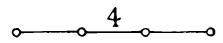
\includegraphics[keepaspectratio]{images/part002_520d8dd1.jpg}}

\begin{enumerate}
\def\labelenumi{(\roman{enumi})}
\setcounter{enumi}{1}
\tightlist
\item
  If the edge \(\{1,2\}\) is of order 5, the graph is one of the following:
\end{enumerate}

\pandocbounded{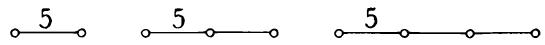
\includegraphics[keepaspectratio]{images/part002_9200390b.jpg}}

We can assume that \(l > 2\) (Lemma 4). Assume that \(\{i, i + 1\}\) is of order \(\geqslant 4\) , with \(1 \leqslant i \leqslant l - 1\) . Put

\(x = e_{1} + 2e_{2} + \dots + ie_{i}, y = e_{l} + 2e_{l - 1} + \dots + (l - i)e_{i + 1},\) and \(j = l - i\) .

By Lemma 8. \(\| x\|^2 = \frac{1}{2} i(i + 1),\| y\|^2 = \frac{1}{2} j(j + 1)\) . On the other hand, \((x|y) = ij(e_i|e_{i + 1}) = -ij\cos \frac{\pi}{m}\) with \(m = 4\) or 5 (Lemma 4). Now

\[
(x | y) ^ {2} <   \left\| x \right\| ^ {2} \| y \| ^ {2}.
\]

which gives

\[
\frac {1}{4} i j (i + 1) (j + 1) > i ^ {2} j ^ {2} \cos^ {2} \frac {\pi}{m}
\]

SO

\[
(i + 1) (j + 1) > 4 i j \cos^ {2} \frac {\pi}{m} \geqslant 2 i j.
\]

This gives, first of all, \(ij - i - j - 1 < 0\) , or \((i - 1)(j - 1) < 2\) . If

\[
1 <   i <   l - 1,
\]

then \(1 < j < l - 1\) , so \(i = j = 2\) , and so \({}^1\)

\[
9 > 16 \cos^ {2} {\frac {\pi}{m}}, \text {thus} \cos^ {2} {\frac {\pi}{m}} <   \cos^ {2} {\frac {\pi}{5}}
\]

and hence \(m = 4\) . This proves (i). If \(i = 1\) and \(m = 5\) , then \(2j + 2 > 4j\frac{3 + \sqrt{5}}{8}\) , or \(j\frac{\sqrt{5} - 1}{2} < 2\) , \(j < \sqrt{5} + 1 < 4\) , and so \(l = j + 1 \leqslant 4\) . This proves (ii).

Lemma 10. If X has a ramification point i, the full subgraph \(X - \{i\}\) is the union of three chains, and if p - 1, q - 1, r - 1 are the lengths of these chains, the triple \(\{p, q, r\}\) is equal, up to a permutation, to one of the triples \(\{1, 2, 2\}\) , \(\{1, 2, 3\}\) , \(\{1, 2, 4\}\) , \(\{1, 1, m\}\) (for some \(m \geqslant 1\) ).

The vertex \(i\) belongs to 3 edges (Lemma 2), and there is no other ramification point (Lemma 7), so the full subgraph \(\mathrm{X} - \{i\}\) is the sum of 3 chains \(\mathrm{X}_1\) , \(\mathrm{X}_2\) , \(\mathrm{X}_3\) each of which has a terminal vertex linked to \(i\) in \(\mathrm{X}\) . Let \(\{i_1, i_2\}\) , \(\{i_2, i_3\}, \ldots, \{i_{p-1}, i_p\}\) be the edges of \(\mathrm{X}_1\) , \(\{j_1, j_2\}\) , \(\{j_2, j_3\}, \ldots, \{j_{q-1}, j_q\}\) those of \(\mathrm{X}_2\) , and \(\{k_1, k_2\}\) , \(\{k_2, k_3\}, \ldots, \{k_{r-1}, k_r\}\) those of \(\mathrm{X}_3\) , with \(i_1, j_1, k_1\) linked to \(i\) in \(\mathrm{X}\) . We can assume that \(p \geqslant q \geqslant r \geqslant 1\) . Put

\[
\begin{array}{l} x = e _ {i _ {p}} + 2 e _ {i _ {p - 1}} + \dots + p e _ {i _ {1}} \\ y = e _ {j _ {q}} + 2 e _ {j _ {q - 1}} + \dots + q e _ {j _ {1}} \\ z = e _ {k _ {r}} + 2 e _ {k _ {r - 1}} + \dots + r e _ {k _ {1}}. \end{array}
\]

Since all the edges of X are of order 3 (Lemma 7), Lemma 8 gives \(\| x\|^2 = \frac{1}{2} p(p + 1)\) , \(\| y\|^2 = \frac{1}{2} q(q + 1)\) , \(\| z\|^2 = \frac{1}{2} r(r + 1)\) . On the other hand, \(e_i\) is orthogonal to \(e_{i_2}, e_{i_3}, \ldots, e_{i_p}\) , so \((e_i|x) = p(e_i|e_{i_1}) = -\frac{1}{2} p\) ; similarly \((e_i|y) = -\frac{1}{2} q\) , \((e_i|z) = -\frac{1}{2} r\) . The unit vectors \(\| x\|^ {-1}x\) , \(\| y\|^ {-1}y\) , \(\| z\|^ {-1}z\) are mutually orthogonal, and \(e_i\) does not belong to the subspace F that they generate; the square of the distance from \(e_i\) to F is

\[
\begin{array}{r l} 1 - (e _ {i} | \frac {x}{\| x \|}) ^ {2} - (e _ {i} | \frac {y}{\| y \|}) ^ {2} - (e _ {i} | \frac {z}{\| z \|}) ^ {2} \\ & = 1 - \frac {1}{2} \frac {p}{p + 1} - \frac {1}{2} \frac {q}{q + 1} - \frac {1}{2} \frac {r}{r + 1} \\ & = 1 - \frac {1}{2} + \frac {1}{2} \frac {1}{p + 1} - \frac {1}{2} + \frac {1}{2} \frac {1}{q + 1} - \frac {1}{2} + \frac {1}{2} \frac {1}{r + 1}. \end{array}
\]

Since this quantity is \(>0\) , we have

\[
(p + 1) ^ {- 1} + (q + 1) ^ {- 1} + (r + 1) ^ {- 1} > 1.\tag{4}
\]

Hence \(3(r + 1)^{-1} > 1\) , so \(r < 2\) and finally \(r = 1\) . Then (4) gives

\[
(p + 1) ^ {- 1} + (q + 1) ^ {- 1} > \frac {1}{2}\tag{5}
\]

hence \(2(q + 1)^{-1} > \frac{1}{2}\) . so \(q \leqslant 2\) . Finally, if \(q = 2\) , (5) gives

\[
(p + 1) ^ {- 1} > \frac {1}{6}. \quad \text { hence } p \leqslant 4.
\]

THEOREM 1. The graph of any irreducible finite Coxeter system (W.S) is isomorphic to one of the following:

\pandocbounded{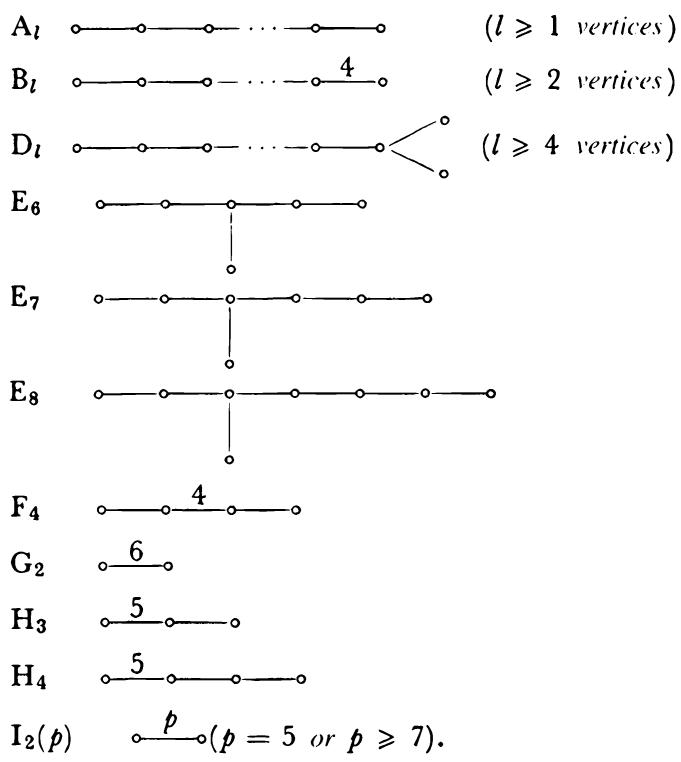
\includegraphics[keepaspectratio]{images/part002_677d99d4.jpg}}

No two of these graphs are isomorphic.

Indeed, let \(\mathrm{W} = (m_{ij})\) be the Coxeter matrix of (W,S), and let \(l = \operatorname{Card}(S)\) . If one of the \(m_{ij}\) is \(\geqslant 6\) , then l = 2 (Lemma 4) and the Coxeter graph of (W,S) is of type \(G_{2}\) or \(I_{2}(p)\) with \(p \geqslant 7\) . Assume now that all the \(m_{ij} \leqslant 5\) .

\begin{enumerate}
\def\labelenumi{\alph{enumi})}
\item
  If the \(m_{ij}\) are not all equal to 3, the graph X of (W.S) is a chain and exactly one of the \(m_{ij}\) is equal to 4 or 5 (Lemma 7). If one of the \(m_{ij}\) is equal to 5, Lemma 9 shows that we have one of the types \(H_{3}\) , \(H_{4}\) or \(I_{2}(5)\) . If one of the \(m_{ij}\) is equal to 4, Lemma 9 shows that we have one of the types \(B_{l}\) or \(F_{4}\) .
\item
  Assume now that all the \(m_{ij}\) are equal to 3. If X is a chain, the Coxeter graph is of type \(A_{l}\) . If not, Lemma 10 shows that it is of type \(E_{6}\) , \(E_{7}\) , \(E_{8}\) or \(D_{l}\) .
\end{enumerate}

The fact that no two of the Coxeter graphs listed are isomorphic is clear.

Conversely:

THEOREM 2. The Coxeter groups defined by the Coxeter graphs \(\mathbf{A}_l, \mathbf{B}_l, \ldots, \mathbf{I}_2(p)\) of Th. 1 are finite.

This is clear for \(I_{2}(p)\) , the corresponding group being the dihedral group of order 2p (Chap. IV, § 1, no. 9). For \(H_{4}\) the corresponding quadratic form

is

\[
\begin{array}{r l} & \xi_ {1} ^ {2} + \xi_ {2} ^ {2} + \xi_ {3} ^ {2} + \xi_ {4} ^ {2} - \xi_ {1} \xi_ {2} - \xi_ {2} \xi_ {3} - 2 (\cos \frac {\pi}{5}) \xi_ {3} \xi_ {4} \\ & = \xi_ {1} ^ {2} + \xi_ {2} ^ {2} + \xi_ {3} ^ {2} + \xi_ {4} ^ {2} - \xi_ {1} \xi_ {2} - \xi_ {2} \xi_ {3} - \frac {1 + \sqrt {5}}{2} \xi_ {3} \xi_ {4} \\ & = (\xi_ {2} - \frac {\xi_ {1} + \xi_ {3}}{2}) ^ {2} + (\xi_ {4} - \frac {1 + \sqrt {5}}{4} \xi_ {3}) ^ {2} + \frac {3}{4} (\xi_ {1} - \frac {1}{3} \xi_ {3}) ^ {2} + \frac {7 - 3 \sqrt {5}}{24} \xi_ {3} ^ {2}. \end{array}
\]

Since \(7 - 3\sqrt{5}\) is \textgreater0, this form is positive non-degenerate, and the corresponding Coxeter group is finite. The same holds for that corresponding to \(H_{3}\) , since it is isomorphic to a subgroup of the preceding (Chap. IV, § 1, no. 8).

For the types \(A_{l}\) , \(B_{l}, \ldots, G_{2}\) , we shall construct, in Nos. 5 to 13, root systems having the corresponding groups as Weyl groups. We shall see that these groups are not only finite, but crystallographic (§ 2, no. 5).

\subsection{DYNKIN GRAPHS}

By abuse of language, we shall call a normed graph a pair \((\Gamma, f)\) having the following properties:

\begin{enumerate}
\def\labelenumi{\arabic{enumi})}
\item
  \(\Gamma\) is a graph (called the underlying graph of \((\Gamma, f)\) ).
\item
  If E denotes the set of pairs \((i,j)\) such that \(\{i,j\}\) is an edge of \(\Gamma\) . f is a map from E to R such that \(f(i,j)f(j,i)=1\) for all \((i,j)\in\mathbf{E}\) .
\end{enumerate}

There is an obvious notion of isomorphism of normed graphs.

Let R be a reduced root system in a real vector space V. We are going to associate to it a normed graph \((X, f)\) , called the Dynkin graph of R. The vertices of X will be the elements of the set I of orbits of W(R) in the union of the sets \(\{B\} \times B\) (where B is the set of bases of R). If \(N = (n_{ij})_{i,j \in I}\) (resp. \(M = (m_{ij})_{i,j \in I}\) ) is the canonical Cartan matrix (resp. the Coxeter matrix) of R ( \(\S\) 1, no. 5, Remark 7), two vertices i and j of X are linked if and only if \(n_{ij} \neq 0\) and we then put

\[
f (i, j) = \frac {n _ {i j}}{n _ {j i}}.
\]

Since \(n_{ij} = 0\) implies \(n_{ji} = 0\) , this defines a normed graph (X. f).

Let \((x|y)\) be a scalar product on V. invariant under W(R), and let \(B = (\alpha_i)_{i \in I}\) be a basis of R. indexed canonically. Formulas (7) and (9) of § 1. no. 1 show that vertices i and j of the graph X are linked if and only if

\[
(\alpha_ {i} | \alpha_ {j}) \neq 0
\]

and that

\[
f (i, j) = \frac {\left(\alpha_ {j} \mid \alpha_ {i}\right)}{\left(\alpha_ {j} \mid \alpha_ {j}\right)}.
\]

In view of the results of § 1, Nos. 3 and 5, the only possibilities are the following, up to interchanging \(i\) and \(j\) :

\begin{enumerate}
\def\labelenumi{\arabic{enumi})}
\item
  \(i\) and \(j\) are not linked; \(n_{ij} = n_{ji} = 0\) ; \(m_{ij} = 2\) ;
\item
  \(f(i,j) = f(j,i) = 1; n_{ij} = n_{ji} = -1; m_{ij} = 3;\)
\item
  \(f(i,j) = 2\) , \(f(j,i) = 1/2\) ; \(n_{ij} = -2\) . \(n_{ji} = -1\) ; \(m_{ij} = 4\) ;
\end{enumerate}

\[
f (i, j) = 3, f (j, i) = 1 / 3: n _ {i j} = - 3, n _ {j i} = - 1; m _ {i j} = 6.
\]

We see from this that the Dynkin graph R determines the Cartan matrix and the Coxeter matrix of R, and hence determines R up to isomorphism. More precisely, the Cor. of Prop. 15 of § 1, no. 5 implies the following result:

PROPOSITION 1. Let \(R_{1}\) and \(R_{2}\) be two reduced root systems in vector spaces \(V_{1}\) and \(V_{2}\) . Let \(B_{1} = (\alpha_{i})_{i \in I_{1}}\) and \(B_{2} = (\alpha_{i})_{i \in I_{2}}\) be bases of \(R_{1}\) and \(R_{2}\) , indexed canonically. Let \(\lambda\) be an isomorphism from the Dynkin graph of \(R_{1}\) to the Dynkin graph of \(R_{2}\) . Then, there exists a unique isomorphism from \(V_{1}\) to \(V_{2}\) transforming \(R_{1}\) into \(R_{2}\) and \(\alpha_{i}\) into \(\alpha_{\lambda(i)}\) for all \(i \in I_{1}\) .

It is clear that an automorphism of R defines an automorphism of the Dynkin graph of R, and hence a homomorphism \(\varphi\) from the group A(R) to the group of automorphisms of the Dynkin graph of R.

COROLLARY. The homomorphism \(\varphi\) defines by passage to the quotient an isomorphism from the group A(R)/W(R) to the group of automorphisms of the Dynkin graph of R.

Clearly, \(\varphi(g) = \operatorname{Id}\) for all \(g \in W(R)\) . On the other hand, Prop. 1 shows that there exists an isomorphism \(\psi\) from the group of isomorphisms of the Dynkin graph of \(R\) to the subgroup \(E\) of elements of \(A(R)\) leaving fixed a given basis \(B\) of \(R\) , such that \(\varphi \circ \psi = \operatorname{Id}\) . Since \(A(R)\) is the semi-direct product of \(E\) and \(W(R)\) (§ 1, no. 5, Prop. 16), the corollary follows.

In practice, the Dynkin graph \((X, f)\) is represented by a diagram composed of nodes and bonds in the following way. The nodes correspond to the vertices of X; two nodes corresponding to two distinct vertices i and j are joined by 0, 1, 2 or 3 bonds in cases 1), 2), 3) and 4) above (up to interchanging i and j). Moreover, in cases 3) and 4), that is when \(f(i, j) > 1\) , or when the roots \(\alpha_{1}\) and \(\alpha_{j}\) are not orthogonal and not of the same length, an inequality sign \textgreater{} is placed on the double or triple bond joining the nodes corresponding to i and j oriented towards the node corresponding to j (that is, the shortest root):

\[
\underset {i} {\longrightarrow} \underset {j} {\longrightarrow} \quad (\text { for   } f (i, j) = 2), \quad \underset {i} {\longrightarrow} \underset {j} {\longrightarrow} \quad (\text { for   } f (i, j) = 3).
\]

It is clear that the Dynkin graph \((X, f)\) can be recovered from this diagram.

We remark that the diagram associated to the Coxeter graph of W(R) can be obtained from that associated to the Dynkin graph of R by keeping the nodes and the single bonds and replacing the double (resp. triple) bonds by a bond surmounted by the number 4 (resp. 6). Conversely, given the Coxeter graph of W(R), the diagram associated to the Dynkin graph of R can be recovered using the inverse of this procedure, except for the inequality signs on the double or triple bonds. Th. 1 thus gives immediately the list of possible Dynkin graphs. More precisely:

THEOREM 3. If R is an irreducible reduced root system, its Dynkin graph is isomorphic to one of the graphs represented by the following diagrams:

\pandocbounded{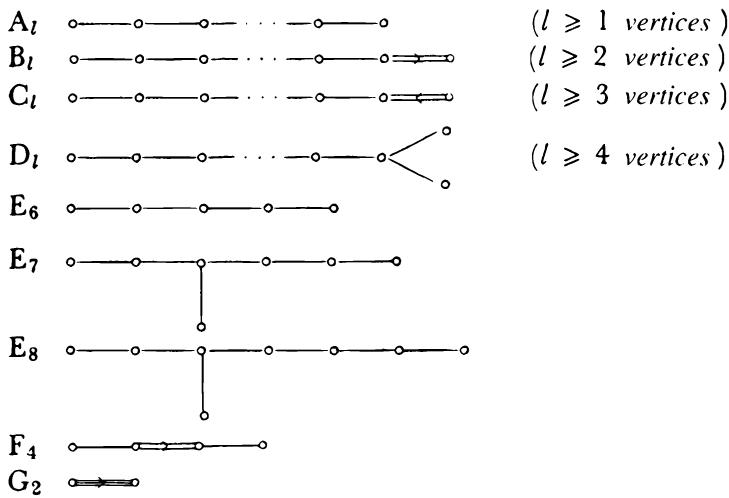
\includegraphics[keepaspectratio]{images/part002_c37a5a77.jpg}}

No two of these graphs are isomorphic and there are irreducible reduced root systems having each of them as their Dynkin graph (up to isomorphism).

The first assertion follows immediately from Th. 1, in view of the preceding remarks, the fact that the Coxeter groups of the graphs \(H_{3}\) , \(H_{4}\) and \(I_{2}(p)\) (for p = 5 and \(p \geqslant 7\) ) are not crystallographic, and the fact that the two possible inequalities for the double (resp. triple) bond of the Dynkin graph associated to the Coxeter graph \(F_{4}\) (resp. \(G_{2}\) ) give isomorphic Dynkin graphs. The second assertion is clear and the third will follow from the explicit construction of an irreducible reduced root system for each type, a construction that will be carried out in Nos. 5 to 13.

Remarks. 1) The graph \(A_{1}\) reduces to a single node; we denote it also by \(B_{1}\) or \(C_{1}\) . The graph \(B_{2}\) is also denoted by \(C_{2}\) . The graph \(A_{3}\) is also denoted by \(D_{3}\) . Finally, \(D_{2}\) denotes the graph consisting of two unconnected nodes. (These conventions are derived from the properties of the corresponding root systems, cf.~nos. 5 to 8.)

\begin{enumerate}
\def\labelenumi{\arabic{enumi})}
\setcounter{enumi}{1}
\tightlist
\item
  If \((X, f)\) is the Dynkin graph of a reduced root system R. the Dynkin graph of the inverse system can be identified with \((X, f^{-1})\) . In other words, the diagram associated to the Dynkin graph of \(R^{\prime}\) can be obtained from that associated to the Dynkin graph of R by reversing the inequality signs. If R is irreducible, we see that R is isomorphic to \(R^{\prime}\) unless R is of type \(B_{l}\) or \(C_{l}\) , in which case \(R^{\prime}\) is of type \(C_{l}\) or \(B_{l}\) .
\end{enumerate}

\subsection{AFFINE WEYL GROUP AND COMPLETED DYNKIN GRAPH}

Let R be an irreducible reduced root system and let \((\mathbf{X}, f)\) be its Dynkin graph. We are going to define another normed graph \((\tilde{\mathbf{X}}, \tilde{f})\) that we shall call the completed Dynkin graph of R. The set \(\tilde{I}\) of vertices of \(\tilde{X}\) consists of the set I of vertices of X and a vertex denoted by 0, not belonging to I. To define \(\tilde{f}\) , choose a basis \(B = (\alpha_{i})_{i \in I}\) of R and a scalar product \((x|y)\) invariant under W(R). Let \(\alpha_{0}\) be the negative of the highest root for the order defined by B. Two distinct vertices \(i, j \in \tilde{I}\) are linked if and only if \((\alpha_{i}|\alpha_{j}) \neq 0\) and we then put

\[
\tilde {f} (i, j) = \frac {\left(\alpha_ {i} \mid \alpha_ {i}\right)}{\left(\alpha_ {j} \mid \alpha_ {j}\right)}.
\]

It is immediate that the graph \(\tilde{X}\) and the map \(\tilde{f}\) thus defined do not depend on the choice of B or the scalar product.

If the rank \(l\) of \(R\) is equal to 1, then \(I = \{i\}\) and \(\alpha_0 = -\alpha_1\) ; hence \(\tilde{f}(0, i) = 1\) . If \(l \geqslant 2\) , \(\alpha_0\) is not proportional to any of the \(\alpha_i\) and \((\alpha_0|\alpha_i)\) is \(\leqslant 0\) (§ 1. no. 8. Prop. 25). For any pair \((i,j)\) of distinct elements of \(\tilde{I}\) , the only possibilities are those denoted by 1), 2), 3), 4) in the preceding number (putting, for example, \(n_{0i} = n(\alpha_0, \alpha_i)\) and \(m_{0i} = \text{order of } s_{\alpha_0}s_{\alpha_i}\) for all \(i \in I\) ).

In the case \(l \geqslant 2\) , the completed Dynkin graph is represented by a diagram with the same conventions as in the preceding number, sometimes indicating by dotted lines the bonds joining the vertex 0 to the other vertices. We remark that the inequality sign \textgreater{} on such a bond, if it exists, is always directed towards the vertex distinct from 0, since \(\alpha_{0}\) is a longest root ( \(\S\) 1, no. 8, Prop. 25). The graph \((\mathbf{X}, f)\) is the subgraph obtained from \((\tilde{\mathbf{X}}, f)\) by deleting the vertex 0.

The action of A(R) on (X. f) extends to an action on \((\tilde{\mathbf{X}}.\tilde{f})\) , leaving 0 fixed, and W(R) acts trivially on \((\tilde{\mathbf{X}}.\tilde{f})\) .

We retain the notations of § 2. Prop. 5 of § 2, no. 2, together with Th. 1 of Chap. V, § 3, no. 2, shows that the Coxeter graph \(\Sigma\) of the affine Weyl group \(W_{a}(R)\) can be obtained from \((\tilde{X},\tilde{f})\) by the same rules by which the Coxeter graph of \(W(R)\) is obtained from \((X,f)\) . On the other hand, let G be the normaliser of \(W_{a}(R)\) (§ 2, no. 3). To any \(g\in G\) corresponds an automorphism \(\varphi(g)\) of \(\Sigma\) and \(\varphi(g)=\mathrm{Id}\) if \(g\in W_{a}(R)\) . Conversely, given an automorphism \(\lambda\) of \(\Sigma\) there is, by Prop. 11 of Chap. V, § 4, no. 9, a unique element \(g=\psi(\lambda)\) preserving a given alcove C and such that \(\varphi(g)=\lambda\) . Since G is the semi-direct product of the subgroup \(G_{C}\) of elements preserving C and \(W_{a}(R)\) (§ 2, no. 3), we deduce that \(\varphi\) defines by passage to the quotient an isomorphism from \(G/W_{a}\) (or from \(G_{C}\) ) to \(\operatorname{Aut}(\Sigma)\) . It is immediate that the composite of this isomorphism with the canonical map from A(R)/W(R) to G/ \(W_{a}\) coincides with the homomorphism from A(R)/W(R) to \(\operatorname{Aut}(\Sigma)\) induced by the homomorphism from A(R)/W(R) to \(\operatorname{Aut}(\tilde{X},\tilde{f})\) defined above. By § 2, no. 3, the group \(\operatorname{Aut}(\Sigma)\) is isomorphic to the semi-direct product of

\(A(R)/W(R)\) by \(P(R')/Q(R')\) , and \(P(R')/Q(R')\) is isomorphic to the group \(I_{C'} = G_{C'} \cap W_{a}'\) (with the notation of § 2. no. 3): the element of \(\text{Aut}(\Sigma)\) corresponding to the element \(\gamma_{i}\) of \(I_{C}\) transforms the vertex 0 to the vertex i of \(\Sigma\) .

Remark. It can be shown that the canonical map

\[
\operatorname{Aut} (\tilde {X}, \tilde {f}) \rightarrow \operatorname{Aut} (\Sigma)
\]

is an isomorphism.

THEOREM 4. Let (W.S) be an irreducible Coxeter system with S finite. The associated quadratic form (Chap. V. § 4, no. 1) is positive and degenerate if and only if the Coxeter graph of (W.S) is isomorphic to one of the following:

\pandocbounded{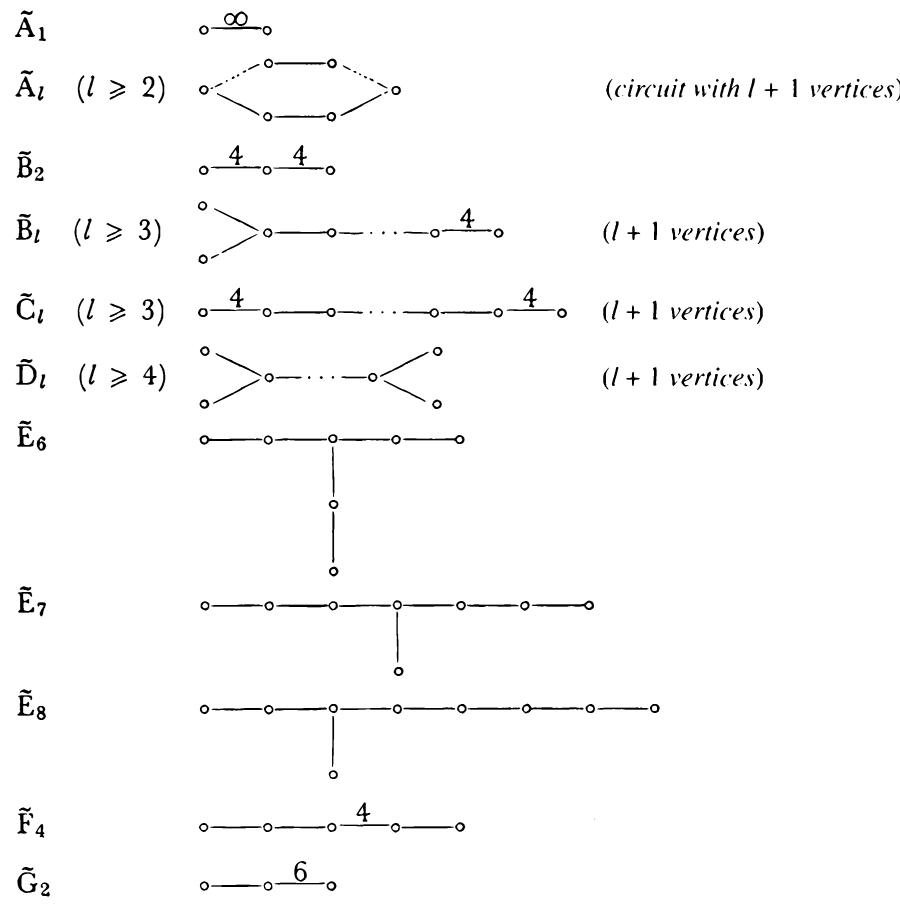
\includegraphics[keepaspectratio]{images/part002_b5f8d83f.jpg}}

No two of these Coxeter graphs are isomorphic.

By Chap. V. § 4, no. 9 and Prop. 8 of § 2, no. 5, the Coxeter systems whose quadratic form is positive and degenerate are those which correspond to the affine Weyl groups of irreducible reduced root systems. The theorem therefore follows from the determination of the completed Dynkin graphs made in nos. 5 to 13 below.

\subsection{PRELIMINARIES TO THE CONSTRUCTION OF ROOT SYSTEMS}

Let V be a real vector space of dimension \(l \geqslant 1\) equipped with a scalar product \((x|y)\) . L a discrete subgroup of V, A a finite set of numbers \textgreater0, and R the set of \(\alpha \in L\) such that \((\alpha|\alpha) \in \Lambda\) . Assume that R generates V and that, for any pair \((\alpha,\beta)\) of points of R, the number \(2\frac{(\alpha|\beta)}{(\alpha|\alpha)}\) is an integer. Then, R is a root system in V. Indeed, R clearly satisfies \((RS_{I})\) . Let \(\alpha \in R\) : let \(s_{\alpha}\) be the orthogonal reflection \(x \mapsto x - 2\frac{(x|\alpha)}{(\alpha|\alpha)}\alpha\) ; then, if \(\beta \in R\) , we have \(2\frac{(\beta|\alpha)}{(\alpha|\alpha)} \in Z\) , so \(s_{\alpha}(\beta) \in L\) , and moreover \(\|s_{\alpha}(\beta)\| = \| \beta \|\) , so \(s_{\alpha}(\beta) \in R\) ; thus, R satisfies \((RS_{II})\) and \((RS_{III})\) , and is reduced if A does not contain two numbers of the form \(\lambda\) and \(4\lambda\) .

Now let V be a subspace of \(E = R^{n}\) . Let \((\varepsilon_{1}, \ldots, \varepsilon_{n})\) be the canonical basis of E; we equip E with the scalar product for which this basis is orthonormal and identify \(E^{*}\) with E (resp. \(V^{*}\) with V) by means of this scalar product. We define subgroups \(L_{0}, L_{1}, L_{2}, L_{3}\) of E as follows:

\begin{enumerate}
\def\labelenumi{\arabic{enumi})}
\item
  \(L_{0}\) is the Z-module with basis \((\varepsilon_{i})\) . We have \((\alpha|\beta)\in\mathbf{Z}\) for all \(\alpha,\beta\in L_{0}\) . The vectors \(\alpha\in L_{0}\) for which \((\alpha|\alpha)=1\) are the \(\pm\varepsilon_{i}\;(1\leqslant i\leqslant n)\) ; those for which \((\alpha|\alpha)=2\) are the \(\pm\varepsilon_{i}\pm\varepsilon_{j}\) for i\textless j (the two signs \(\pm\) , in \(\pm\varepsilon_{i}\pm\varepsilon_{j}\) , are chosen independently of each other; we adopt an analogous convention throughout the remainder of this section).
\item
  \(L_{1}\) is the Z-submodule of \(L_{0}\) consisting of the \(x = \sum_{i=1}^{n} \xi_{i} \varepsilon_{i} \in L_{0}\) such that \(\sum_{i=1}^{n} \xi_{i}\) is even; since \(\xi_{i}\) and \(\xi_{i}^{2}\) have the same parity, this is equivalent to requiring that \((x|x)\) is even. Let \(L_{1}^{\prime}\) be the submodule of \(L_{1}\) generated by the \(\varepsilon_{i} \pm \varepsilon_{j}\) ; we have \(\sum_{i=1}^{n} \xi_{i} \varepsilon_{i} \equiv (\sum_{i=1}^{n} \xi_{i}) \varepsilon_{n} \pmod{L_{1}^{\prime}}\) , and since \(2\varepsilon_{n} = (\varepsilon_{1} + \varepsilon_{n}) - (\varepsilon_{1} - \varepsilon_{n}) \in L_{1}^{\prime}\) , it follows that \(L_{1}^{\prime} = L_{1}\) . Since \(L_{0}\) is generated by \(L_{1}\) and \(\varepsilon_{1}, L_{0}/L_{1}\) is isomorphic to Z/2Z.
\item
  \(\mathrm{L}_2 = \mathrm{L}_0 + \mathbf{Z}\left(\frac{1}{2} \sum_{i=1}^{n} \varepsilon_i\right)\) . It is clear that an element \(x = \sum_{i=1}^{n} \xi_i \varepsilon_i\) of \(\mathrm{V}\) is in \(\mathrm{L}_2\) if and only if
\end{enumerate}

\[
2 \xi_ {i} \in \mathbf {Z}, \quad \xi_ {i} - \xi_ {j} \in \mathbf {Z} \text {   for   all   } i \text {   and   } j.\tag{6}
\]

Since \((\varepsilon_k|_{\frac{1}{2}}\sum_{i=1}^{n}\varepsilon_i) = \frac{1}{2}\) for all \(k\) , and since \(\| \frac{1}{2}\sum_{i=1}^{n}\varepsilon_i\|^2 = \frac{n}{4}\) , we have \((\alpha|\beta) \in \frac{1}{2}\mathbf{Z}\) for \(\alpha, \beta \in L_2\) if \(n\) is even. The group \(L_2 / L_0\) is isomorphic to \(\mathbf{Z}/2\mathbf{Z}\) .

\begin{enumerate}
\def\labelenumi{\arabic{enumi})}
\setcounter{enumi}{3}
\tightlist
\item
  \(L_{3} = L_{1} + \mathbf{Z}\left(\frac{1}{2} \sum_{i=1}^{n} \varepsilon_{i}\right)\) . If n is a multiple of 4, \(L_{3}\) is the set of \(\sum_{i=1}^{n} \xi_{i} \varepsilon_{i}\) satisfying (6) and the condition \(\sum_{i=1}^{n} \xi_{i} \in 2\mathbf{Z}\) : in this case, \((\alpha | \beta) \in \mathbf{Z}\) for all \(\alpha, \beta \in L_{3}\) .
\end{enumerate}

It is immediate that the subgroup of E associated to \(L_{0}\) (resp. \(L_{1}, L_{2}\) ) is \(L_{0}\) (resp. \(L_{2}, L_{1}\) ). The subgroup of E associated to \(L_{3}\) is the set of

\[
x = \sum_ {i = 1} ^ {n} \xi_ {i} \varepsilon_ {i} \in L _ {2}
\]

such that \((x|\frac{1}{2}\sum_{i = 1}^{n}\varepsilon_i)\in \mathbf{Z}\) , that is, such that \(\sum_{i = 1}^{n}\xi_{i}\in 2\mathbf{Z}\) : if \(n\equiv 0\) (mod. 4), this associated subgroup is therefore \(\mathrm{L}_3\) .

The abelian group \(\mathrm{L}_2 / \mathrm{L}_1\) is of order 4, and hence is isomorphic to \(\mathbf{Z} / 4\mathbf{Z}\) or \(\mathbf{Z} / 2\mathbf{Z} \times \mathbf{Z} / 2\mathbf{Z}\) (Algebra, Chap. VII, § 4, no. 6, Th. 3). If \(n\) is odd,

\[
p (\frac {1}{2} \sum_ {i = 1} ^ {n} \varepsilon_ {i}) \in \mathrm{L} _ {1} \Leftrightarrow p \equiv 0 (\mathrm{mod.} 4)
\]

so \(\mathrm{L}_2 / \mathrm{L}_1\) is cyclic of order 4. If \(n\) is even,

\[
p (\frac {1}{2} \sum_ {i = 1} ^ {n} \varepsilon_ {i}) \in \mathrm{L} _ {1} \Leftrightarrow p \equiv 0 (\mathrm{mod.} 2)
\]

so \(L_{2}/L_{1}\) , which contains two distinct elements of order 2, is isomorphic to \(Z/2Z \times Z/2Z\) .

We shall use this notation throughout the next nine nos. and in the plates. For each type of Dynkin graph in Th. 3, we shall describe explicitly:

\begin{enumerate}
\def\labelenumi{(\Roman{enumi})}
\item
  A root system R and the number of roots.
\item
  A basis B of R. and the corresponding positive roots. The basis B will be indexed by the integers \(1,\ldots,l\) .
\item
  The Coxeter number \(h\) (§ 1. no. 11).
\item
  The highest root \(\tilde{\alpha}\) (for the order defined by B) and the completed Dynkin graph (no. 3). We shall indicate next to each vertex the corresponding root of B.
\item
  The inverse system \(\mathbb{R}^{\prime}\) , the canonical bilinear form and the constant \(\gamma(\mathbb{R})\) (§ 1, no. 12).
\item
  The fundamental weights relative to B (§ 1, no. 10).
\item
  The sum of the positive roots.
\item
  The groups \(P(R), Q(R), P(R)/Q(R)\) and the connection index (§ 1, no. 9).
\item
  The exponents of \(\mathrm{W}(\mathrm{R})\) (Chap. V. § 6, no. 2, Def. 2). In the cases \(\mathbf{A}_l, \mathbf{B}_l, \mathbf{C}_l\) and \(\mathbf{D}_l\) we determine the symmetric invariants.
\item
  The order of W(R) (and in some cases its structure).
\item
  The group \(A(R)/W(R)\) , its action on the Dynkin graph, and the element \(w_{0}\) of \(W(R)\) that transforms B to -B.
\item
  The action of \(\mathrm{P}(\mathrm{R}^{\prime})/\mathrm{Q}(\mathrm{R}^{\prime})\) on the completed Dynkin graph and the action of \(\mathrm{A}(\mathrm{R})/\mathrm{W}(\mathrm{R})\) on \(\mathrm{P}(\mathrm{R}^{\prime})/\mathrm{Q}(\mathrm{R}^{\prime})\) .
\end{enumerate}

For each Dynkin graph in Th. 3, these data will be collected in Plates I to IX, and ordered in a uniform way as above. We also give:

\begin{enumerate}
\def\labelenumi{(\Roman{enumi})}
\setcounter{enumi}{12}
\tightlist
\item
  The Cartan matrix, from which the Dynkin graph is derived as described in no. 2.
\end{enumerate}

\subsection{\texorpdfstring{SYSTEMS OF TYPE \(B_{l}\) (\(l \geqslant 2\))}{SYSTEMS OF TYPE B\_l (l >= 2)}}

\begin{enumerate}
\def\labelenumi{(\Roman{enumi})}
\item
  We consider the group \(L_{0}\) in V = \(R^{l}\) (no. 4). Let R be the set of \(\alpha \in L_{0}\) such that \((\alpha|\alpha) = 1\) or \((\alpha|\alpha) = 2\) , in other words the set of vectors \(\pm\varepsilon_{i}\) ( \(1 \leqslant i \leqslant l\) ) and \(\pm\varepsilon_{i} \pm \varepsilon_{j}\) ( \(1 \leqslant i < j \leqslant l\) ). It is clear that R generates V and that \(2(\alpha|\beta)/(\alpha|\alpha) \in \mathbf{Z}\) for all \(\alpha, \beta \in R\) . Thus R is a reduced root system in V (no. 4). The number of roots is \(n = 2l + 4\frac{l(l-1)}{2} = 2l^{2}\) .
\item
  Put
\end{enumerate}

\[
\alpha_ {1} = \varepsilon_ {1} - \varepsilon_ {2}, \alpha_ {2} = \varepsilon_ {2} - \varepsilon_ {3}, \dots , \alpha_ {l - 1} = \varepsilon_ {l - 1} - \varepsilon_ {l}, \alpha_ {l} = \varepsilon_ {l}.
\]

Then

\[
\begin{array}{c} \varepsilon_ {i} = \alpha_ {i} + \alpha_ {i + 1} + \dots + \alpha_ {l} \quad (1 \leqslant i \leqslant l) \\ \varepsilon_ {i} + \varepsilon_ {j} = (\alpha_ {i} + \alpha_ {i + 1} + \dots + \alpha_ {l}) + (\alpha_ {j} + \alpha_ {j + 1} + \dots + \alpha_ {l}) (1 \leqslant i <   j \leqslant l) \\ \varepsilon_ {i} - \varepsilon_ {j} = \alpha_ {i} + \alpha_ {i + 1} + \dots + \alpha_ {j - 1} \quad (1 \leqslant i <   j \leqslant l). \end{array}
\]

Thus \((\alpha_{1},\alpha_{2},\ldots ,\alpha_{l})\) is a basis of R (§ 1, no. 7. Cor. 3 of Prop. 20). Moreover, \(\| \alpha_{i}\|^{2} = 2\) for \(i < l\) , \(\| \alpha_l\| ^2 = 1\) , \((\alpha_i|\alpha_{i + 1}) = -1\) for \(1\leqslant i\leqslant l - 1\) , \((\alpha_i|\alpha_j) = 0\) for \(j > i + 1\) : the Dynkin graph of R is thus of type \(\mathbf{B}_l\) , which shows that R is irreducible. The positive roots are the \(\varepsilon_{i}\) and the \(\varepsilon_{i}\pm \varepsilon_{j}\) ( \(i < j\) ).

\begin{enumerate}
\def\labelenumi{(\Roman{enumi})}
\setcounter{enumi}{2}
\tightlist
\item
  By Th. 1 (ii) of Chap. V, § 6, no. 2.
\end{enumerate}

\[
h = n / l = 2 l.
\]

\begin{enumerate}
\def\labelenumi{(\Roman{enumi})}
\setcounter{enumi}{3}
\tightlist
\item
  Let \(\tilde{\alpha} = \varepsilon_{1} + \varepsilon_{2} = \alpha_{1} + 2\alpha_{2} + 2\alpha_{3} + \cdots + 2\alpha_{l}\) , which is a root. The sum of its coordinates relative to the basis \((\alpha_{i})\) is 2l - 1 = h - 1. In view of Prop. 31 of § 1, no. 11, \(\tilde{\alpha}\) is the highest root of R. We have \((\tilde{\alpha}| \alpha_{i}) = 0\) for \(i \neq 2\) and \((\tilde{\alpha}| \alpha_{2}) = 1\) . Since \(\alpha_{2}\) is of length 1 (resp. \(\sqrt{2}\) ) when l = 2 (resp. \(l \geqslant 3\) ), the completed Dynkin graph of R is as follows:
\end{enumerate}

\[
\text { for } l = 2 \quad \alpha_ {2} \alpha_ {1}
\]

\pandocbounded{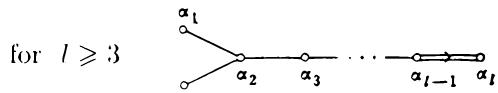
\includegraphics[keepaspectratio]{images/part002_79c781e2.jpg}}

\begin{enumerate}
\def\labelenumi{(\Alph{enumi})}
\setcounter{enumi}{21}
\tightlist
\item
  The formula \(\alpha^{\prime} = \frac{2\alpha}{(\alpha|\alpha)}\) gives for \(R^{\prime}\) the set of vectors \(\pm 2\varepsilon_{i}\) ( \(1 \leqslant i \leqslant l\) ), \(\pm \varepsilon_{i} \pm \varepsilon_{j}\) ( \(1 \leqslant i < j \leqslant l\) ). The Dynkin graph of \(R^{\prime}\) is obtained from that of \(R\) by the procedure explained in no. 2, and we see that \(R^{\prime}\) is of type \(C_{l}\) .
\end{enumerate}

There are \(4l - 2\) roots not orthogonal to \(\beta = \varepsilon_1\) , namely \(\pm \varepsilon_1\) and \(\pm \varepsilon_1 \pm \varepsilon_j\) for \(2 \leqslant j \leqslant l\) ; for each such root \(\alpha\) , \(n(\alpha, \beta) = \pm 2\) . Formula (17) of § 1, no. 12 shows that, for \(\Phi_{\mathrm{R}}\) , the square of the length of \(\beta\) is \((4l - 2)^{-1}\) ; hence \(\Phi_{\mathrm{R}}(x, y) = (x|y)/(4l - 2)\) . Apply formula (18) of § 1, no. 12 with \(x = y = \beta\) . This gives

\[
2 + \frac {1}{4} (4 l - 4) = \gamma (R) \frac {1}{4 l - 2}
\]

and so \(\gamma(R) = (l + 1)(4l - 2)\) .

\begin{enumerate}
\def\labelenumi{(\Roman{enumi})}
\setcounter{enumi}{5}
\tightlist
\item
  The fundamental weights \(\omega_{i}\) ( \(1 \leqslant i \leqslant l\) ) such that \((\omega_{i}|\alpha_{j}) = \delta_{ij}\) are easily calculated, and we find that
\end{enumerate}

\[
\begin{array}{l} \omega_ {i} = \varepsilon_ {1} + \varepsilon_ {2} + \dots + \varepsilon_ {i} \\ \qquad = \alpha_ {1} + 2 \alpha_ {2} + \dots + (i - 1) \alpha_ {i - 1} + i (\alpha_ {1} + \alpha_ {i + 1} + \dots + \alpha_ {l}) (i <   l) \\ \omega_ {l} = \frac {1}{2} (\varepsilon_ {1} + \varepsilon_ {2} + \dots + \varepsilon_ {l}) = \frac {1}{2} (\alpha_ {1} + 2 \alpha_ {2} + \dots + l \alpha_ {l}). \end{array}
\]

\begin{enumerate}
\def\labelenumi{(\Roman{enumi})}
\setcounter{enumi}{6}
\tightlist
\item
  The sum of the positive roots is
\end{enumerate}

\[
\begin{array}{l} 2 \rho = (2 l - 1) \varepsilon_ {1} + (2 l - 3) \varepsilon_ {2} + \dots + 3 \varepsilon_ {l - 1} + \varepsilon_ {l} \\ = (2 l - 1) \alpha_ {1} + 2 (2 l - 2) \alpha_ {2} + \dots + i (2 l - i) \alpha_ {i} + \dots + l ^ {2} \alpha_ {l}. \end{array}
\]

\begin{enumerate}
\def\labelenumi{(\Roman{enumi})}
\setcounter{enumi}{7}
\item
  We have \(Q(R) = L_{0}\) (no. 4), and \(P(R)\) is generated by \(Q(R)\) and \(\omega_{l}\) , hence is equal to \(L_{2}\) (no. 4). Hence, \(P(R)/Q(R)\) is isomorphic to Z/2Z, and the connection index is equal to 2.
\item
  and (X) In \(R^{l}\) , the orthogonal reflection \(s_{\varepsilon_{i}-\varepsilon_{j}}\) ( \(i \neq j\) ) interchanges \(\varepsilon_{i}\) and \(\varepsilon_{j}\) and leaves \(\varepsilon_{k}\) invariant when the index k is distinct from i and j. The \(s_{\varepsilon_{i}-\varepsilon_{j}}\) generate a group \(G_{1}\) isomorphic to the symmetric group \(S_{l}\) . The orthogonal reflection \(s_{\varepsilon_{i}}\) transforms \(\varepsilon_{i}\) to \(-\varepsilon_{i}\) and leaves invariant the \(\varepsilon_{k}\) when the index k is distinct from i. The \(s_{\varepsilon_{i}}\) generate a group \(G_{2}\) isomorphic to \((\mathbf{Z}/2\mathbf{Z})^{l}\) . The Weyl group W(R) is generated by \(G_{1}\) and \(G_{2}\) , and \(G_{2}\) is normal in W(R), so W(R) is isomorphic to the semi-direct product of \(S_{l}\) by \((\mathbf{Z}/2\mathbf{Z})^{l}\) . Its order is therefore \(2^{l}\cdot l!\) .
\end{enumerate}

The symmetric algebra \(\mathbf{S}(\mathbf{R}^{l})\) can be identified canonically with the algebra of polynomial functions \(\mathrm{P}(\xi_{1},\ldots,\xi_{l})\) on \(R^{l}\) . For such a polynomial to be invariant under \(\mathrm{W}(\mathrm{R})\) , it is first of all necessary that

\[
P \left(\xi_ {1}. \xi_ {2}. \dots ., \xi_ {l}\right) = P \left(\pm \xi_ {1}. \pm \xi_ {2}. \dots ., \pm \xi_ {l}\right)
\]

for all choices of the signs on the right-hand side, so that

\[
\mathrm{P} \left(\xi_ {1}, \dots , \xi_ {l}\right) = \mathrm{Q} \left(\xi_ {1} ^ {2}, \dots , \xi_ {l} ^ {2}\right)
\]

where Q is a polynomial, and further that Q is a symmetric polynomial; and these conditions are sufficient. Consequently (Algebra. Chap. V, App. I), \(\mathbf{S}(\mathbf{R}^{l})^{\mathrm{W}(\mathbb{R})}\) is the algebra generated by the l polynomial functions

\[
t _ {i} = \sum_ {\tau \in \mathfrak {S} _ {l}} \xi_ {\tau (1)} ^ {2} \xi_ {\tau (2)} ^ {2} \dots \xi_ {\tau (l)} ^ {2} \quad (1 \leqslant i \leqslant l).
\]

Moreover, the transcendence degree over \(\mathbf{R}\) of the field of fractions of \(\mathbf{S}(\mathbf{R}^l)^{\mathrm{W(R)}}\) is \(l\) , so the \(t_i\) are algebraically independent. Since the \(t_i\) have degree \(2,4,\ldots ,2l\) , we conclude that the exponents of \(\mathrm{W(R)}\) (Chap. V. § 6, no. 3, Prop. 3) are:

\[
1, 3, 5, \dots , 2 l - 1.
\]

\begin{enumerate}
\def\labelenumi{(\Roman{enumi})}
\setcounter{enumi}{10}
\item
  The only automorphism of the Dynkin graph is the identity element. Thus, \(A(R) = W(R)\) and \(-1 \in W(R)\) . Since -1 transforms B to -B, we conclude that \(w_{0} = -1\) .
\item
  The group \(P(R^{\prime})/Q(R^{\prime})\) is dual to \(P(R)/Q(R)\) , and hence is isomorphic to Z/2Z. Its non-trivial element permutes the vertices corresponding to \(\alpha_{0}\) and \(\alpha_{1}\) and leaves the others fixed.
\end{enumerate}
